\documentclass[10pt,twocolumn,letterpaper]{article}

\usepackage{iccv}
\usepackage{times}
\usepackage{epsfig}
\usepackage{graphicx}
\usepackage{amsmath}
\usepackage{amssymb}
\usepackage{multirow}
\usepackage{diagbox}
\usepackage{amsmath,booktabs}

%\usepackage[colorlinks,urlcolor=black]{hyperref}
%\usepackage{cite}
% Include other packages here, before hyperref.

% If you comment hyperref and then uncomment it, you should delete
% egpaper.aux before re-running latex.  (Or just hit 'q' on the first latex
% run, let it finish, and you should be clear).
\usepackage[pagebackref=true,breaklinks=true,letterpaper=true,colorlinks,bookmarks=false]{hyperref}

\iccvfinalcopy % *** Uncomment this line for the final submission

\def\iccvPaperID{2799} % *** Enter the ICCV Paper ID here
\def\httilde{\mbox{\tt\raisebox{-.5ex}{\symbol{126}}}}

% Pages are numbered in submission mode, and unnumbered in camera-ready
\ificcvfinal\pagestyle{empty}\fi
\begin{document}

%%%%%%%%% TITLE
%\title{PU-GAN: a Point cloud Upsampling Generative Adversarial Network}
%\title{PU-GAN: a Point cloud Unpsampling Adversarial Network}
%\title{PU-GAN: Point Cloud Upsampling using a Generative Adversarial Network}
\title{PU-GAN: a Point Cloud Upsampling Adversarial Network}

\author{Ruihui Li$^{1}$\quad Xianzhi Li$^{1,3}$\quad Chi-Wing Fu$^{1,3}$\quad Daniel Cohen-Or$^2$\quad Pheng-Ann Heng$^{1,3}$\\
	%$^1$Department of Computer Science and Enginering \hspace{10mm} $^2$School of Computer Science,\\
	\hspace{-10mm}$^1$The Chinese University of Hong Kong \hspace{10mm} $^2$ Tel Aviv University\\
	$^3$Guangdong Provincial Key Laboratory of Computer Vision and Virtual Reality Technology,\\
	Shenzhen Institutes of Advanced Technology, Chinese Academy of Sciences, China\\
	\hspace{-10mm}{\tt\small \{lirh,xzli,cwfu,pheng\}@cse.cuhk.edu.hk}\hspace{10mm}{\tt\small dcor@mail.tau.ac.il}\qquad
}
\newcommand{\TODO}[1]{{\color{red}{[TODO: #1]}}}
\newcommand{\phil}[1]{{\color[rgb]{0.3,0.7,0.3}{[PH: #1]}}}
%\newcommand{\rh}[1]{{\color{blue}{#1}}}
\newcommand{\rh}[1]{#1}
\newcommand{\xz}[1]{{\color[rgb]{1.0,0.6,0}{[XZ: #1]}}}
\newcommand{\dc}[1]{{\color{red}{[DC: #1]}}}
\newcommand{\para}[1]{\vspace{.05in}\noindent\textbf{#1}}
\def\ie{\emph{i.e.}}
\def\eg{\emph{e.g.}}
\def\etal{{\em et al.}}
\def\etc{{\em etc.}}

\maketitle
%\thispagestyle{empty}


\begin{abstract}
Point clouds acquired from range scans are often sparse, noisy, and non-uniform.
%, as can be seen in various 3D benchmarks.
%
%\dc{do we really need to bring the benchmarks as a proof? i would just make the claim, it is obvious}
This paper presents a new point cloud upsampling network called PU-GAN \footnote[1]{\href{https://liruihui.github.io/publication/PU-GAN/}{https://liruihui.github.io/publication/PU-GAN/}}, which is formulated based on a generative adversarial network (GAN), to learn a rich variety of point distributions from the latent space and upsample points over patches on object surfaces.
%
%To realize a working GAN network, we design an up-down-up expansion unit in the generator to upsample per-point features with %error feedback and self-correction, and formulate a self-attention unit to enhance the feature integration.
%\dc{since we did not invent the up-down-up, I suggest the following}
%\phil{Our up-down-up is different from the image one... Fig.3}
To realize a working GAN network, we construct an up-down-up expansion unit in the generator for upsampling point features with error feedback and self-correction, and formulate a self-attention unit to enhance the feature integration.
%
Further, we design a compound loss with adversarial, uniform and reconstruction terms, to encourage the discriminator to learn more latent patterns and enhance the output point distribution uniformity.
%\dc{where? not clear why ``discover'', maybe ``learn''?}.
%\phil{actually, XZ and RH follow a GAN paper to use the word "discover", but learn is ok
%
Qualitative and quantitative evaluations demonstrate the quality of our results over the state-of-the-arts in terms of distribution uniformity, proximity-to-surface, and 3D reconstruction quality.
%
%Both qualitative and quantitative comparison results against recent methods demonstrate the quality of our results over the state-of-the-art methods in terms of distribution uniformity, proximity-to-surface, and 3D reconstruction quality.
%\dc{the abstract does not sell the key point of why ``GAN'' is so helpful here. I feel that you feel uneasy to claim that the losses alone cannot deliver the work}
%
%To encourage the upsampled points to locate on the underlying surface with a uniform distribution, we further formulate loss terms to guide the learning of the generator and discriminator.
%\phil{to revise}
%Further, we formulate the uniform loss to improve the distribution uniformity of the points produced by the generator to encourage the discriminator to learn more latent patterns.
%\phil{this sentence is not a good summary of sec 3.5}
%
%To make the GAN framework feasible and capable for the upsampling task, we further introduce a series of adaptations that lead to a substantial performance boost, including a uniform loss, an up-and-down unit, an attention module, etc.
%
%
%We evaluate our method by qualitative and quantitative comparison results, in terms of visual quality, proximity-to-surface, and distribution uniformity, demonstrate the capability of PU-GAN over very recent works on point cloud upsampling and consolidation.
%outperforms the optimization-based, as well as state-of-the-art deep-learning-based approaches, particularly in terms of handling sparse, non-uniform inputs and revealing a complete and uniform point distribution.
\end{abstract}

%\begin{abstract}
%	Point clouds scanned by customer-level devices are typically sparse, noisy, incomplete and non-uniform.
%	To address these issues and generate a high-quality point cloud, in this paper, we propose a novel generative adversarial network (GAN) based point cloud upsampling framework, namely PU-GAN, to learn multimodal structure of the target distribution, for which a simple variational approximation is infeasible.
%	To make the GAN framework feasible and capable for the upsampling task, we further introduce a series of adaptations that lead to a substantial performance boost, including a uniform loss, an up-and-down unit, an attention module, etc.
%	Qualitative and quantitative experimental results show that our PU-GAN significantly outperforms the optimization-based, as well as state-of-the-art deep-learning-based approaches, particularly in terms of handling sparse, non-uniform inputs and revealing a complete and uniform point distribution.
%\end{abstract}

\section{Introduction}
\label{sec:intro}

\begin{figure}[!t]
	\centering
	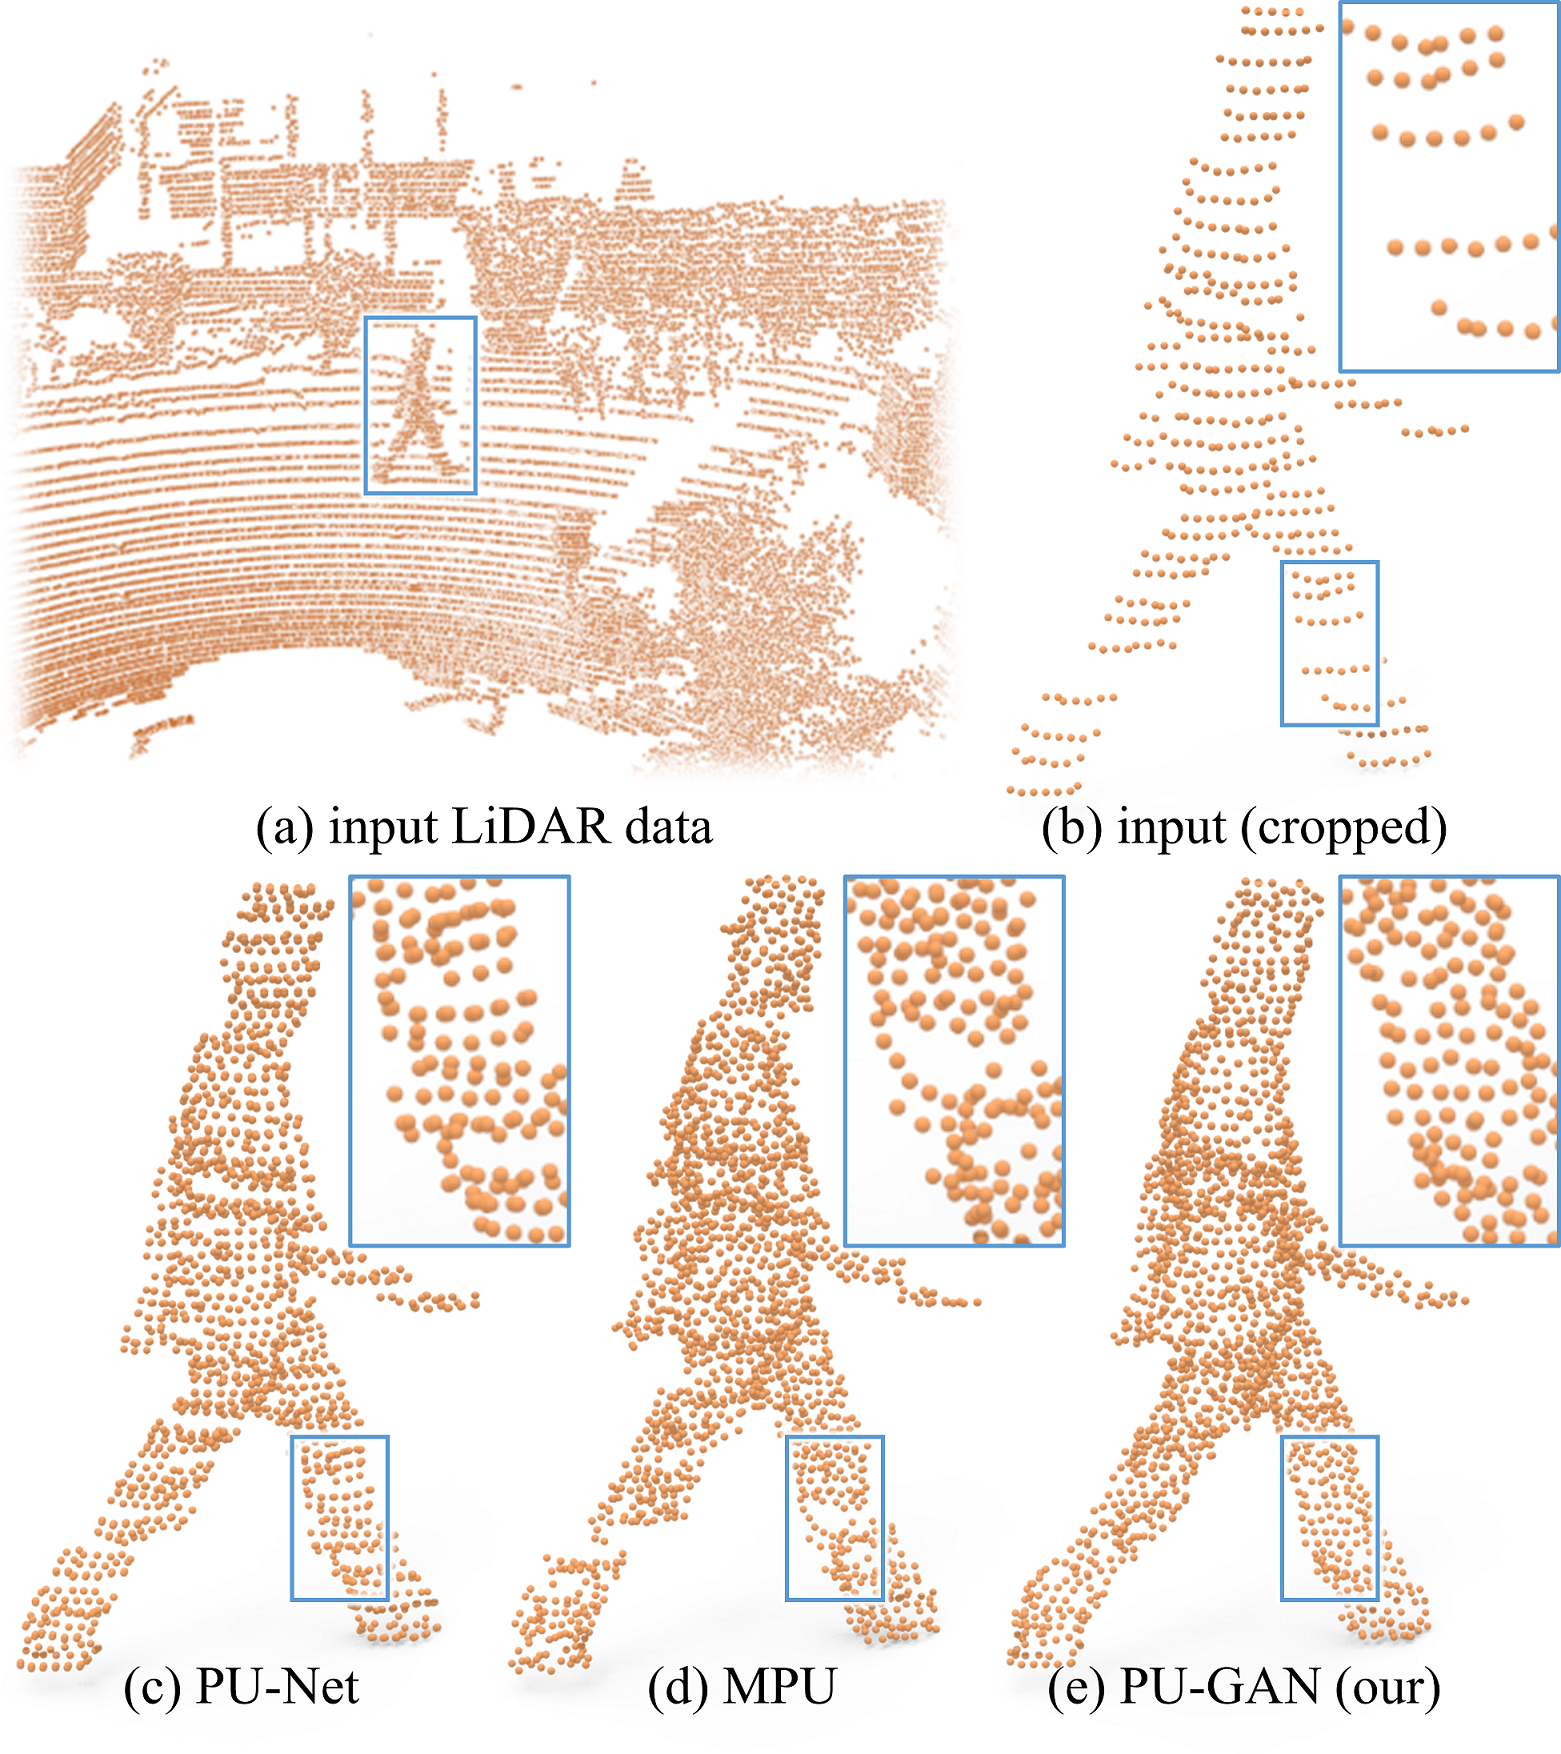
\includegraphics[width=0.95\linewidth]{teaser}
	\caption{Upsampling (b) a point set cropped from (a) the real-scanned KITTI dataset~\cite{geiger2013vision} by using (c) PU-Net~\cite{yu2018pu} (CVPR 2018), (d) MPU~\cite{yifan2018patch} (CVPR 2019), and (e) our PU-GAN.
%The input (b) is cropped from the real-scanned KITTI dataset~\cite{geiger2013vision}.
Note the distribution non-uniformity and sparsity in the input.}
%The input is cropped from a real-scanned LiDAR data, the KITTI dataset~\cite{geiger2013vision}.}
	\label{fig:teaser}
	\vspace*{-2mm}
\end{figure}

% definition of point cloud
%Point cloud is a popular means to represent and process 3D geometry, due to its compactness and generality, as well as due to the fact that it is a standard output from 3D scanning.
% with depth cameras and LiDARs sensors.
%\dc{I suggest the following instead of the above}
Point clouds are the standard outputs from 3D scanning.
In recent years, they are gaining more and more popularity as a compact representation for 3D data, and as an effective means for processing 3D geometry.
%
However, raw point clouds produced from depth cameras and LiDAR sensors are often sparse, noisy, and non-uniform.
This is evidenced in various public benchmark datasets, such as KITTI~\cite{geiger2013vision}, SUN RGB-D~\cite{song2015sun}, and ScanNet~\cite{dai2017scannet}.
Clearly, the raw data is required to be amended, before it can be effectively used for rendering, analysis, or general processing.

%good-quality point clouds without these issues are highly demanded by many applications like rendering, surface reconstruction, and object recognition.

%,~\eg, high-resolution surfel-based point set rendering, surface reconstruction, autonomous navigation, virtual reality,~\etc.
%
%\phil{XZ: please show these applications with comparison at the end of paper}

% definition of point cloud upsampling
%Currently, there are various public benchmarks on point clouds,~\eg, KITTI~\cite{Geiger2012CVPR}, SUN RGB-D~\cite{song2015sun}, ScanNet~\cite{dai2017scannet},~\etc.
%However, these point sets scanned by customer-level devices are typically sparse, noisy and incomplete.
%Thus, point cloud upsampling is particularly necessary.

Given a sparse, noisy, and non-uniform point cloud, our goal is to upsample it and generate a point cloud that is \emph{dense}, \emph{complete}, and \emph{uniform}, as a faithful representation of the underlying surface.
%, without small holes in the results.
%
These goals are very challenging to achieve, given such an imperfect input, since, apart from upsampling the data, we need to fill small holes and gaps in data, while improving the point distribution uniformity.
%; see Figure~\ref{fig:teaser}.
%
%Particularly, we
%\emph{uniformly} and \emph{completely} located on the underlying geometry.
%Different from shape completion, point cloud upsampling does not aim to reconstruct large missing parts and structures that are absent in the input, but it should have the ability to fill in small holes that are caused by the very sparse and non-uniform point distribution.
%However, it is quite challenging to meet the above requirements due to the unordered and irregular properties of 3D points.
%This upsampling problem is quite challenging because the generated dense points should not only describe the underlying geometry of a latent target object, but also have a uniform distribution and roughly cover the complete object surface.
%Hence, simply inserting new points between original points is insufficient.

% current methods and limitations
Early methods~\cite{alexa2003computing,lipman2007parameterization,huang2009consolidation,huang2013edge,wu2015deep} for the problem
%of upsampling and consolidating point clouds
are optimization-based, where various shape priors are used to constrain the point cloud generation.
%
Recently, deep neural networks brought the promise of data-driven approaches to the problem.
Network architectures, including PU-Net~\cite{yu2018pu}, EC-Net~\cite{yu2018ec}, and very recently, MPU~\cite{yifan2018patch}, have demonstrated the advantage of upsampling point clouds through learning.
%
%However, these networks may not be able to produce good results from low-quality inputs (particularly those acquired from real 3D scanning) that are sparse, noisy, and non-uniform; see Figure~\ref{fig:teaser} (c)-(e) for a comparison.
%\dc{I suggest a finer and more careful claim, instead of the above:}
%
However, these networks may not produce plausible results from low-quality inputs that are particularly sparse and non-uniform;
in Figure~\ref{fig:teaser} (c)-(e), we show a typical example that demonstrates the advantage of our method, which unlike the other networks, it combines completion and uniformity together with upsampling.

%generate a complete and uniform point cloud given a very non-uniform sparse point set as input; see Figure~\ref{fig:teaser} (b-c) as examples.

%Most of the existing methods upsample points by solving some kind of optimization, which is commonly constrained by the shape priors~\cite{alexa2003computing,lipman2007parameterization,huang2009consolidation,huang2013edge,wu2015deep}.
%These optimization-based methods, however, tend to yield poor performance when the priors or assumptions are not satisfied.
%Recently, deep learning brings the promise of the data-driven approach.
%Network architectures like PU-Net~\cite{yu2018pu}, EC-Net~\cite{yu2018ec}, and MPU~\cite{yifan2018patch} are successful at upsampling sparse points.
%However, these networks cannot generate a complete and uniform point cloud given a very non-uniform sparse point set as input; see Figure~\ref{fig:teaser} (b-c) as examples.

%\if 0
%% the success of GANs in the field of image processing
%Recently, the generative adversarial network (GAN) has shown its feasibility and capability for image super-resolution with %photo-realistic effect~\cite{ledig2017photo,wu2017srpgan,yuan2018unsupervised,wang2018fully}.
%The key to GAN's success is the idea of an adversarial loss that forces the generated images to be, in principle, %indistinguishable from real photos~\cite{zhu2017unpaired}.
%Naturally, also as a generation task, point cloud upsampling may benefit from such idea of GAN, since we can employ the %adversarial loss to force the generated points to have a uniform distribution.
%However, the adaption of GAN-based techniques to point cloud upsampling is far from straightforward.
%\fi

% our work
%In this work, we present a new point cloud upsampling framework, namely PU-GAN, based on the generative adversarial net (GAN).
%
In this work, we present a new point cloud upsampling framework, namely PU-GAN, that combines upsampling with data amendment capability.
The key contribution is an adversarial network to enable us to train a generator network to learn to produce a rich variety of point distributions from the latent space, and also a discriminator network to help implicitly evaluate the point sets produced from the generator against the latent point distribution.
Particularly, the adversarial learning strategy of the GAN framework can regularize the predictions from a global perspective and implicitly penalize outputs that deviate from the target.
%\phil{I avoided to talk too much about the loss and talk about bypassing the loss, since we also need a loss with several terms (may look complicated) in our method}


%that bypass the need to guide the reconstruction by carefully designed losses. Using a

%GAN framework enables training a generator network generating} a richer variety of point distributions from the latent space, as well as to train a discriminative network to implicitly evaluate the point sets produced from the generator against the true point set distribution. \dc{What is ``true''???}. ...against plausible examples that are dense, complete and have a uniform distribution.
%avoid the necessity of explicitly designing a loss function to guide the generation of point clouds, and on the other hand, to implicitly learn a rich variety of point distributions.
%Particularly, we sidestep the necessity of an explicit loss to directly guide the point set generation, since designing such a loss is hard for our problem, which aims not only for a dense and complete point set but also for a uniform point distribution.
%\dc{It is a bit of repetition, but never mind}
%Particularly, it is hard to design an ideal loss for our problem, where we aim not only for a dense and complete point cloud but also for the point distribution uniformity.
% without direct knowledge of the underlying distribution.

However, successfully training a working GAN framework is known to be challenging~\cite{goodfellow2014distinguishability,radford2015unsupervised}, particularly the difficulty to balance between the generator and discriminator and to avoid the tendency of poor convergence.
%converging to a poor model.
%
Thus, we first improve the point generation quality, or equivalently the feature expansion capability, of the generator, by constructing an up-down-up unit to expand point features by upsampling also their differences for self-correction.
Besides, we formulate a self-attention unit to enhance the feature integration quality.
Lastly, we further design a compound loss to train the network end-to-end with adversarial, uniform, and reconstruction terms to enhance the distribution uniformity of the results and encourage the discriminator to learn more latent patterns in the target distribution.


%
%In this work, we present a novel generative adversarial network (GAN) based framework for point cloud upsampling, namely PU-GAN.
%Compared with manually designing a loss to model the ``ideal'' distribution, we only need to provide ground truth exmaples and the GAN framework can learn multimodal structure of the target distribution, for which a simple variational approximation is infeasible.
%generate the dense points automatically without any priors or constraints.
%As shown in Figure~\ref{fig:teaser} (a), the input real-scanned LiDAR point cloud is very sparse and non-uniform.
%Even under such severe case, our PU-GAN still generates a dense result with complete and uniform point distribution; see Figure~\ref{fig:teaser} (d).

%However, the convergence of training GAN is still an open challenge~\cite{goodfellow2014distinguishability} since it is hard to balance the ablities of the generator and the discriminator during training.
%For instance, if the generator fails to learn the patterns of the target distribution, the discriminator can perfectly distinguish the generated distribution from the target~\cite{arjovsky2017towards}, thus leading to the complete stop of the training process.
%The discriminator must first transfer the new patterns to the generator and then the latter will generate more realistic samples to challenge the former.
%Hence, to make the GAN framework feasible and capable for this upsampling task, we further introduce the following adaptations.
%First, we introduce a novel uniform loss to improve the uniformity of the generated distribution.
%This can promote the training of the discriminator.
%Second, to enhance the feature embedding ability of both generator and discriminator, we further present an up-and-down unit for %error feedback and self-correcting, as well as a self-attention module.
%Last but not least, we merge the farthest sampling into the generator to make the generated points more uniform.

To evaluate the upsampling quality of PU-GAN, we employ four metrics to assess its performance against the state-of-the-arts on a variety of synthetic and real-scanned data.
Extensive experimental results show that our method outperforms others in terms of distribution uniformity, proximity-to-surface, and 3D reconstruction quality.

%To demonstrate the quality of upsampling results, we employ four evaluation metrics to assess the performance of our PU-GAN against the state-of-the-arts using a variety of synthetic and real-scanned data.
%The extensive experiments show that our method outperforms others in terms of distribution uniformity, proximity-to-surface, and 3D reconstruction quality.
%The extensive experiments show that our method compares favorably with others and particularly, the results generated by our PU-GAN are more uniform both locally and globally.

%Specifically, we employ the generator to consume sparse points as input and produce a dense point set (or fake point set).
%We then feed the fake point set into the discriminator to determine if it has the same uniform distribution as the ground truth.
%Note that we consider the points generated by Poisson disk sampling algorithm as the ground truth, since such point distribution has blue noise pattern and is generally considered ideal for many applications~\cite{cook1986stochastic}.

\if 0
Overall, our contributions are summarized below:
\begin{itemize}
	\item
	To the best of our knowledge, we are the first to propose a GAN-based point cloud upsampling network.
	\item
	We propose a series of adaptations for network architecture, including an up-and-down unit with error feedback mechanism, a self-attention module for feature extraction, and the insertion of the farthest sampling into the network structure.
	\item
	We introduce a joint loss function for end-to-end training. Particularly, we propose a novel uniform loss to encourage the upsampled points with a uniform distribution.
\end{itemize}
\fi


\section{Related Work}
\label{sec:bg}



%%%%%%%%%%%%%%%%%%%%%%%%%%%%%%%%%%%%%%%%%%%

\para{Optimization-based upsampling.} \
To upsample a point set, a pioneering method by Alexa~\etal~\cite{alexa2003computing} inserts points at Voronoi diagram vertices in the local tangent space.
%%
Later, Lipman~\etal~\cite{lipman2007parameterization} introduced the locally optimal projection (LOP) operator to resample points and reconstruct surfaces based on an $L_1$ norm.
%, which is able to produce plausible results, even under noise and outliers.
%%
Soon after, Huang~\etal~\cite{huang2009consolidation} devised a weighted LOP with an iterative normal estimation to consolidate point sets with noise, outliers, and non-uniformities.
Huang~\etal~\cite{huang2013edge} further developed a progressive method called EAR for edge-aware resampling of point sets.
%
Later, Wu~\etal~\cite{wu2015deep} proposed a consolidation method to fill large holes and complete missing regions by introducing a new deep point representation.
%%
Overall, these methods are {\em not\/} data-driven; they heavily rely on priors,~\eg, the assumption of smooth surface, normal estimation,~\etc

\begin{figure*}[t]
	\centering
	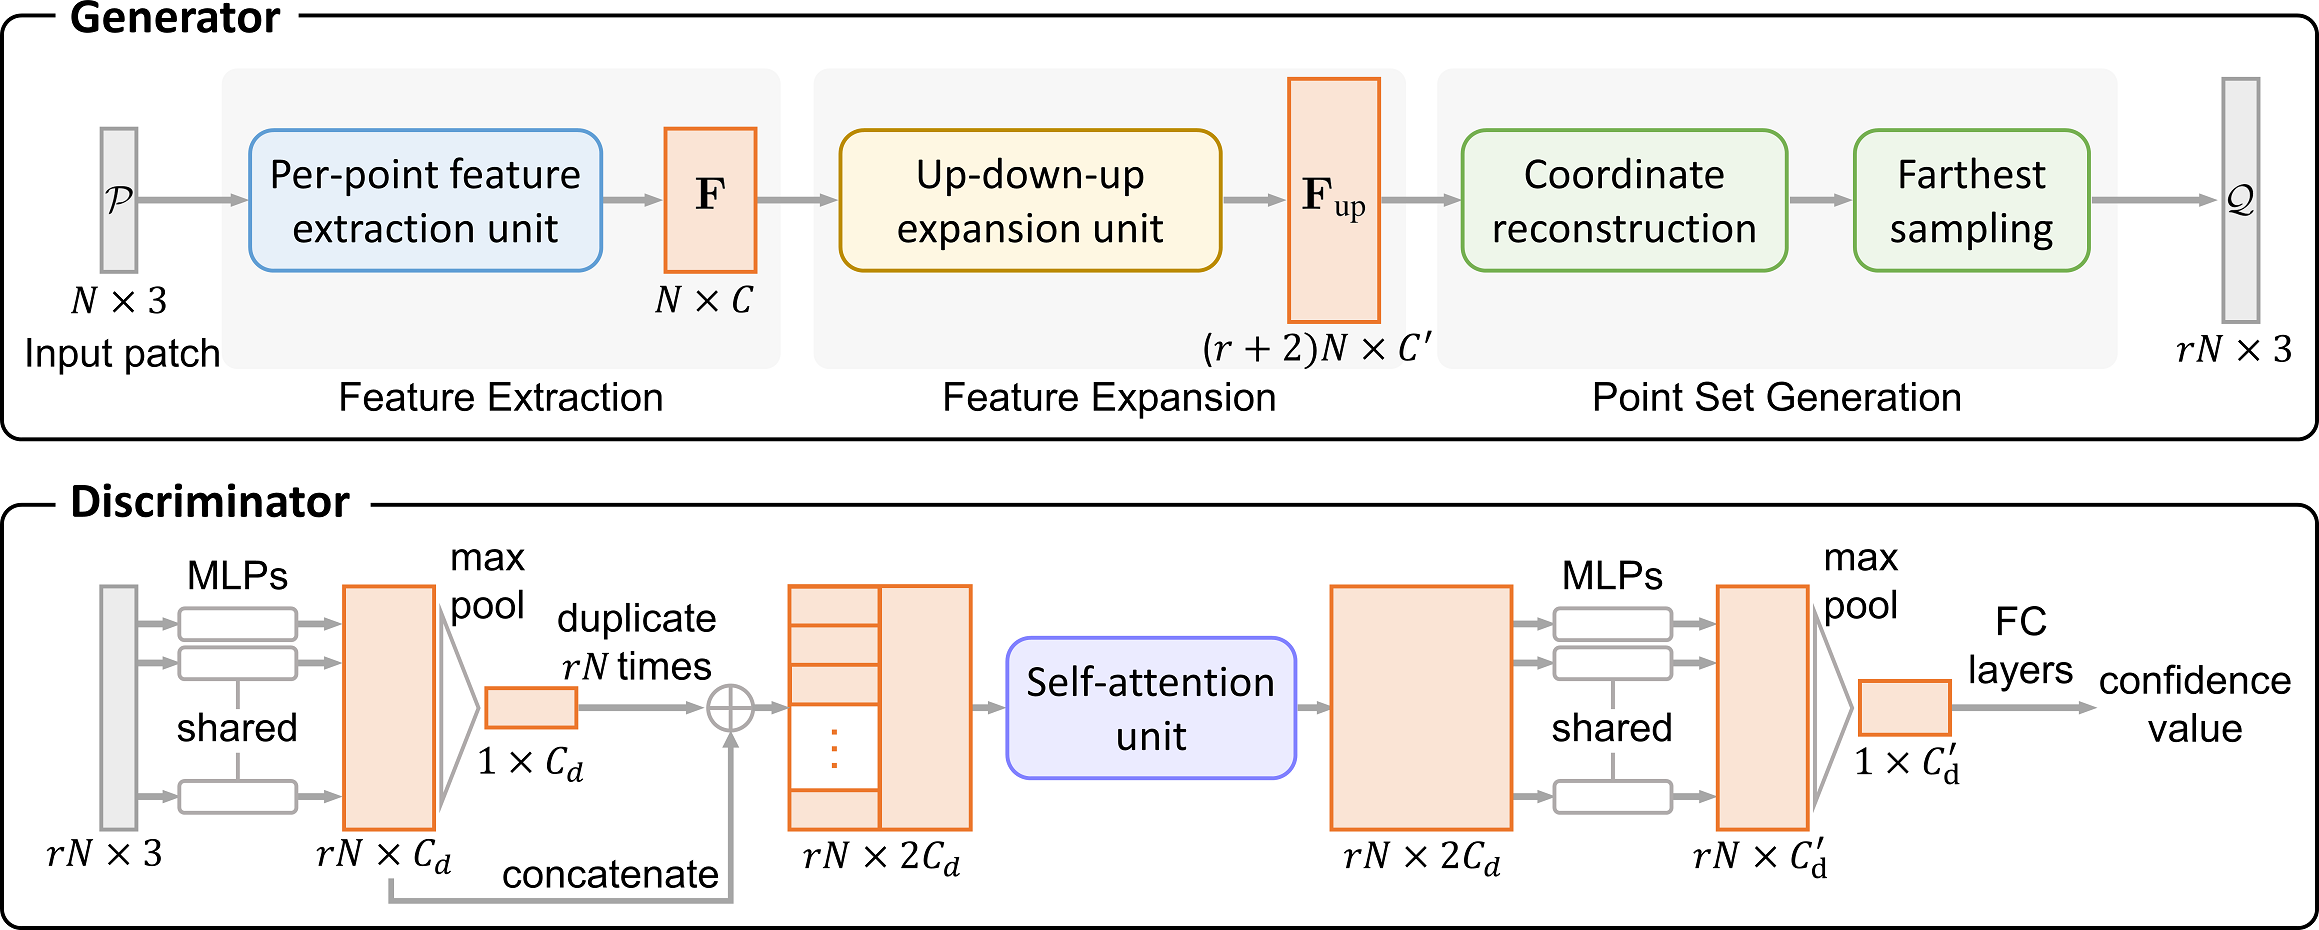
\includegraphics[width=0.88\linewidth]{framework}
	\caption{Overview of PU-GAN's generator and discriminator architecture.
Note that $N$ is the number of points in input $\mathcal{P}$; $r$ is the upsampling rate; and $C$, $C'$, $C_d$, and $C_d'$ are the number of feature channels that are 480, 128, 64, and 256, respectively, in our implementation.}
	\label{fig:framework}
	\vspace*{-2mm}
\end{figure*}

%%%%%%%%%%%%%%%%%%%%%%%%%%%%%%%%%%%%%%%%%%%

\para{Deep-learning-based upsampling.} \
%\phil{XZ: a very short paragraph here to talk about and mention various works on deep feature learning on point cloud}
In recent few years, several deep neural networks have been designed to learn features directly from point sets,~\eg, PointNet~\cite{qi2016pointnet}, PointNet++~\cite{qi2017pointnet++}, SpiderCNN~\cite{xu2018spidercnn}, KCNet~\cite{shen2018mining}, SPLATNet~\cite{su2018splatnet}, PointCNN~\cite{li2018pointcnn}, PointConv~\cite{hua2017pointwise}, PointWeb~\cite{zhao2019pointweb}, DGCNN~\cite{wang2018dynamic}, \emph{etc}.
\rh{Different from point completion ~\cite{yuan2018pcn,gurumurthy2019high} which
generates the entire object from partial input, point cloud upsampling tends to improve the point distribution uniformity within local patches.}
Based on the PointNet++ architecture, Yu~\etal~\cite{yu2018pu} introduced a deep neural network PU-Net to upsample point sets.
PU-Net works on patches and expands a point set by mixing-and-blending point features in the feature space.
Later, they introduced EC-Net~\cite{yu2018ec} for edge-aware point cloud upsampling by formulating an edge-aware joint loss function to minimize the point-to-edge distances.
%regressing a point-to-surface distance and minimizing the point-to-edge losses.
%
Very recently, Wang~\etal~\cite{yifan2018patch} presented a multi-step progressive upsampling (MPU) network to further suppress noise and retain details.
%while He~\etal~\cite{he2019geonet} developed a geodesic neighborhood estimation network GeoNet by fusing the learned geodesic-aware representations into PU-Net.
%
In this work, we present a new method to upsample point clouds by formulating a GAN framework, enabling us to generate higher-quality point samples with completion and uniformity.

%\phil{What is he2019geonet? If we mention it here like this, we have to compare with it quantitatively}



%%%%%%%%%%%%%%%%%%%%%%%%%%%%%%%%%%%%%%%%%%%

%\para{Deep feature learning on point sets.} \
%%
%The advent of fast 3D point cloud acquisition and rapid advances in 3D sensing encourage the development of deep feature learning on point sets.
%%
%Qi~\etal~\cite{qi2016pointnet} introduced the first deep learning network, PointNet, that consumes point sets directly; in particular, its variant PointNet++~\cite{qi2017pointnet++} uses a hierarchical feature learning architecture to capture both local and global geometry context.
%%
%Subsequently, many other networks were proposed for better feature embedding,~\eg, pointwise convolution~\cite{hua2017pointwise}, SpiderCNN~\cite{xu2018spidercnn}, PointGrid~\cite{le2018pointgrid}, KCNet~\cite{shen2018mining}, SPLATNet~\cite{su2018splatnet}, PointCNN~\cite{li2018pointcnn}, DGCNN with EdgeConv block~\cite{wang2018dynamic},~\etc.

\para{GAN-based 3D shape processing.} \
%\phil{(1) start this paragraph by describing the key advantage or strength of GAN over conventional CNN... this helps!}
%\phil{(2) can you shorten the contents below?}
Compared with the conventional CNN, the GAN framework makes use of a discriminator to implicitly learn to evaluate the point sets produced from the generator.
%avoid the need of explicitly designing a loss function to evaluate the network output.
%
Such flexibility particularly benefits generative tasks~\cite{ledig2017photo,isola2017image,zhang2017stackgan}, since we hope the generator can produce a rich variety of output patterns.
%it is often difficult to formulate a perfect loss function.
%\phil{did we get rid of an explicit supervision? if not, need to change the sentence as follows:}
%Such flexibility particularly benefits generative tasks\phil{cite some works on GAN here?}, where ...
%
%Compared with the conventional CNN, by using GAN, we do not need to explicitly design a loss function to evaluate the network output.
%This will undoubtedly bring lots of benefits to these generative-related tasks, because it is often difficult to design a perfect loss function in these tasks.

Recently, there are some inspiring works in applying GAN to 3D shape processing.
Most of them focus on generating 3D objects either from a probabilistic space~\cite{wu2016learning} or from 2D images~\cite{yang20173d,gwak2017weakly,smith2017improved}.
Moreover, Wang~\etal~\cite{wang2017shape} introduced a 3D-ED-GAN for shape completion given a corrupted 3D scan as input.
However, these methods can only consume 3D volumes as inputs or output shapes in voxel representations.
%
Achlioptas~\etal~\cite{achlioptas2018learning} first adapted the GAN model to operate on raw point clouds for enhancing the representation learning.
%superior reconstruction quality.
%However, they mainly focus on representation learning.
%\phil{can its network be adopted to point set upsampling? do we need to compare with this work?}
%
To the best of our knowledge, no prior works develop GAN models for point cloud upsampling.
%\phil{can we really say so, given~\cite{achlioptas2018learning} and the works here?}
%\xz{yes, we can. That work is totally different from us. It has no relationship to upsampling.}

\section{Method}
\label{sec:method}

\subsection{Overview}
\label{subsec:overview}
Given an unordered sparse point set $\mathcal{P}=\{p_i\}_{i=1}^N$ of $N$ points, we aim to generate a dense point set $\mathcal{Q}=\{q_i\}_{i=1}^{rN}$ of $rN$ points, where $r$ is the upsampling rate.
While output $\mathcal{Q}$ is not necessarily a superset of $\mathcal{P}$, we want it to satisfy two requirements:
%\begin{itemize}
%\item
(i) $\mathcal{Q}$ should describe the {\em same underlying geometry\/} of a latent target object as $\mathcal{P}$, so points in $\mathcal{Q}$ should lie on and cover the target object surface; and
%\item
(ii) points in $\mathcal{Q}$ should be {\em uniformly-distributed\/} on the target object surface, even for sparse and non-uniform input $\mathcal{P}$.
%\phil{I assume that you have explained in the intro. why it is good to be uniform... efficiency in representation and good for rendering and meshing}
%\end{itemize}

%\if 0
%\phil{if we cannot do edge-aware at the moment, mention in the limitation?}
%%
%The challenges of the problem are that we not only have to synthesize more points, while ensuring them to lie on the target object surface, but also to deal with the input point set, which can be sparse and non-uniform.
%Particularly, we also aim to improve the uniformity in the generated point set, meaning that we have to deliberately put points in sparse regions and avoid points in dense areas.
%
%In our work, we design a novel GAN-based framework, namely PU-GAN, for point cloud upsampling.
%\fi
Figure~\ref{fig:framework} shows the overall network architecture of PU-GAN, where the generator produces dense output $\mathcal{Q}$ from sparse input $\mathcal{P}$,
% to try to fool the discriminator $D$,
and the discriminator aims to find the fake generated ones.
% from the provided points with uniform distribution.
Following, we first elaborate on the architecture of the generator and discriminator (Section~\ref{subsec:network}).
We then present two building blocks in our architecture: the up-down-up expansion unit (Sections~\ref{subsec:projection}) and the self-attention unit (Section~\ref{subsec:attention}).
Lastly, we present the patch-based training strategy with the compound loss (Section~\ref{subsec:training}).



%%%%%%%%%%%%%%%%%%%%%%%%%%%%%%%%%%%%%%%%%%%%%%%%%%%%%%%%%%%

\subsection{Network Architecture}
\label{subsec:network}

\subsubsection{Generator}
%Our generator consists of three components, including feature extraction, feature expansion, and point set generation; see the top branch in Figure~\ref{fig:framework}.
As shown on top of Figure~\ref{fig:framework}, our generator network has three components to successively process input $\mathcal{P}$:

\para{The feature extraction component} aims to extract features $\mathbf{F}$ from input $\mathcal{P}$ of $N \times d$, where $d$ is the number of dimensions in the input point attributes,~\ie, coordinates, color, normal,~\etc\
Here, we focus on the simplest case with $d=3$, considering only the 3D coordinates, and adopt the recent feature extraction method in~\cite{yifan2018patch}, where dense connections are introduced to integrate features across different layers.
%
%The choice of the feature extraction is flexible and most of the recent works can be employed~\cite{qi2017pointnet++,hua2017pointwise,xu2018spidercnn,shen2018mining,su2018splatnet,li2018pointcnn,wang2018dynamic,yifan2018patch}.
%Here we
%Experimentally, we did not find a significant performance boost on different feature extraction choices; see our supplementary material for experimental results.\TODO{}

\para{The feature expansion component} expands $\mathbf{F}$ to produce the expanded features $\mathbf{F_{\text{up}}}$; here, we design the \emph{up-down-up expansion unit} (see Figure~\ref{fig:framework} (top)) to enhance the feature variations in  $\mathbf{F_{\text{up}}}$, enabling the generator to produce more diverse point distributions; see Section~\ref{subsec:projection} for details.

\para{The point set generation component} first regresses a set of 3D coordinates from $\mathbf{F_{\text{up}}}$ via a set of multilayer perceptrons (MLPs).
%
Since the feature expansion process is still local, meaning that the features in $\mathbf{F_{\text{up}}}$ (or equivalently, points in the latent space) are intrinsically close to the inputs, we thus include a farthest sampling step in the network to retain only $rN$ points that are further away from one another; see the green boxes in Figure~\ref{fig:framework}.
To allow this selection, when we expand $\mathbf{F}$ to $\mathbf{F_{\text{up}}}$, we actually generate $(r+2)N$ features in  $\mathbf{F_{\text{up}}}$.
This strategy further enhances the point set distribution uniformity, particularly from a global perspective.
%
%However, since the feature expansion component has no density-aware ability, thus it will not only add points in sparse regions, but also in the dense regions.
%To address this issue and achieve global uniform, we integrate the farthest sampling into the point set generation component.
%In detail, instead of setting the upsampling rate to be $r$ in the feature expansion component, we set it to be $r+2$, and then apply the farthest sampling to retain $rN$ points.

\subsubsection{Discriminator}
The goal of the discriminator is to distinguish whether its input (a set of $rN$ points) is produced by the generator.
To do so, we first adopt the basic network architecture in~\cite{yuan2018pcn} to extract the global features, since it efficiently combines the local and global information, and ensures a lightweight network.
%
To improve the feature learning, we add a self-attention unit (see Section~\ref{subsec:attention}) after the feature concatenation; see the middle part in Figure~\ref{fig:framework} (bottom).
Compared with the basic MLPs, this attention unit helps enhance the feature integration and improve the subsequent feature extraction capability.
%To enforce complicated geometric constraints on the global point distribution, we introduce a self-attention unit into the discriminator, which enables to check that highly details features in distant portions of the points are consistent with each other. (see Section~\ref{subsec:attention} for details)
%\phil{why at this point inside the discriminator? why not at other point? add some explanation?}
%in the discriminator to enhance the feature integration;
%see the bottom branch in Figure~\ref{fig:framework}.
%
Next, we apply a set of MLPs and a max pooling to produce the global features, and further regress the final confidence value via a set of fully connected layers.
If this confidence value is close to 1, the discriminator predicts that the input likely comes from a target distribution with high confidence, and otherwise from the generator.% vice versa.
%On the other hand, if it is close to 0, the input likely comes from the generator.



%%%%%%%%%%%%%%%%%%%%%%%%%%%%%%%%%%%%%%%%%%%%%%%%%%%%%%%%%%%

\subsection{Up-down-up Expansion Unit}
\label{subsec:projection}
To upsample a point set, PU-Net~\cite{yu2018pu} duplicates the point features and uses separate MLPs to process each copy independently.
However, the expanded features would be too similar to the inputs, so affecting the upsampling quality.
%so due to the one-step feature expansion and may lead to clustered points around the original points.
%
Rather than a single-step expansion, the very recent MPU method~\cite{yifan2018patch} breaks a $16$$\times$ upsampling network into four successive $2$$\times$ upsampling subnets to progressively upsample in multiple steps.
Though details are better preserved in the upsampled results, the training process is complex and requires more subsets for a higher upsampling rate.
%the number of subsets increases with the upsampling rate.
%,~\eg, the subnets have to trained one by one sequentially.
%the scale of the network increases with the upsampling rate.
%\phil{TODO: revise this sentence to make it more specific}

\begin{figure}[!t]
	\centering
	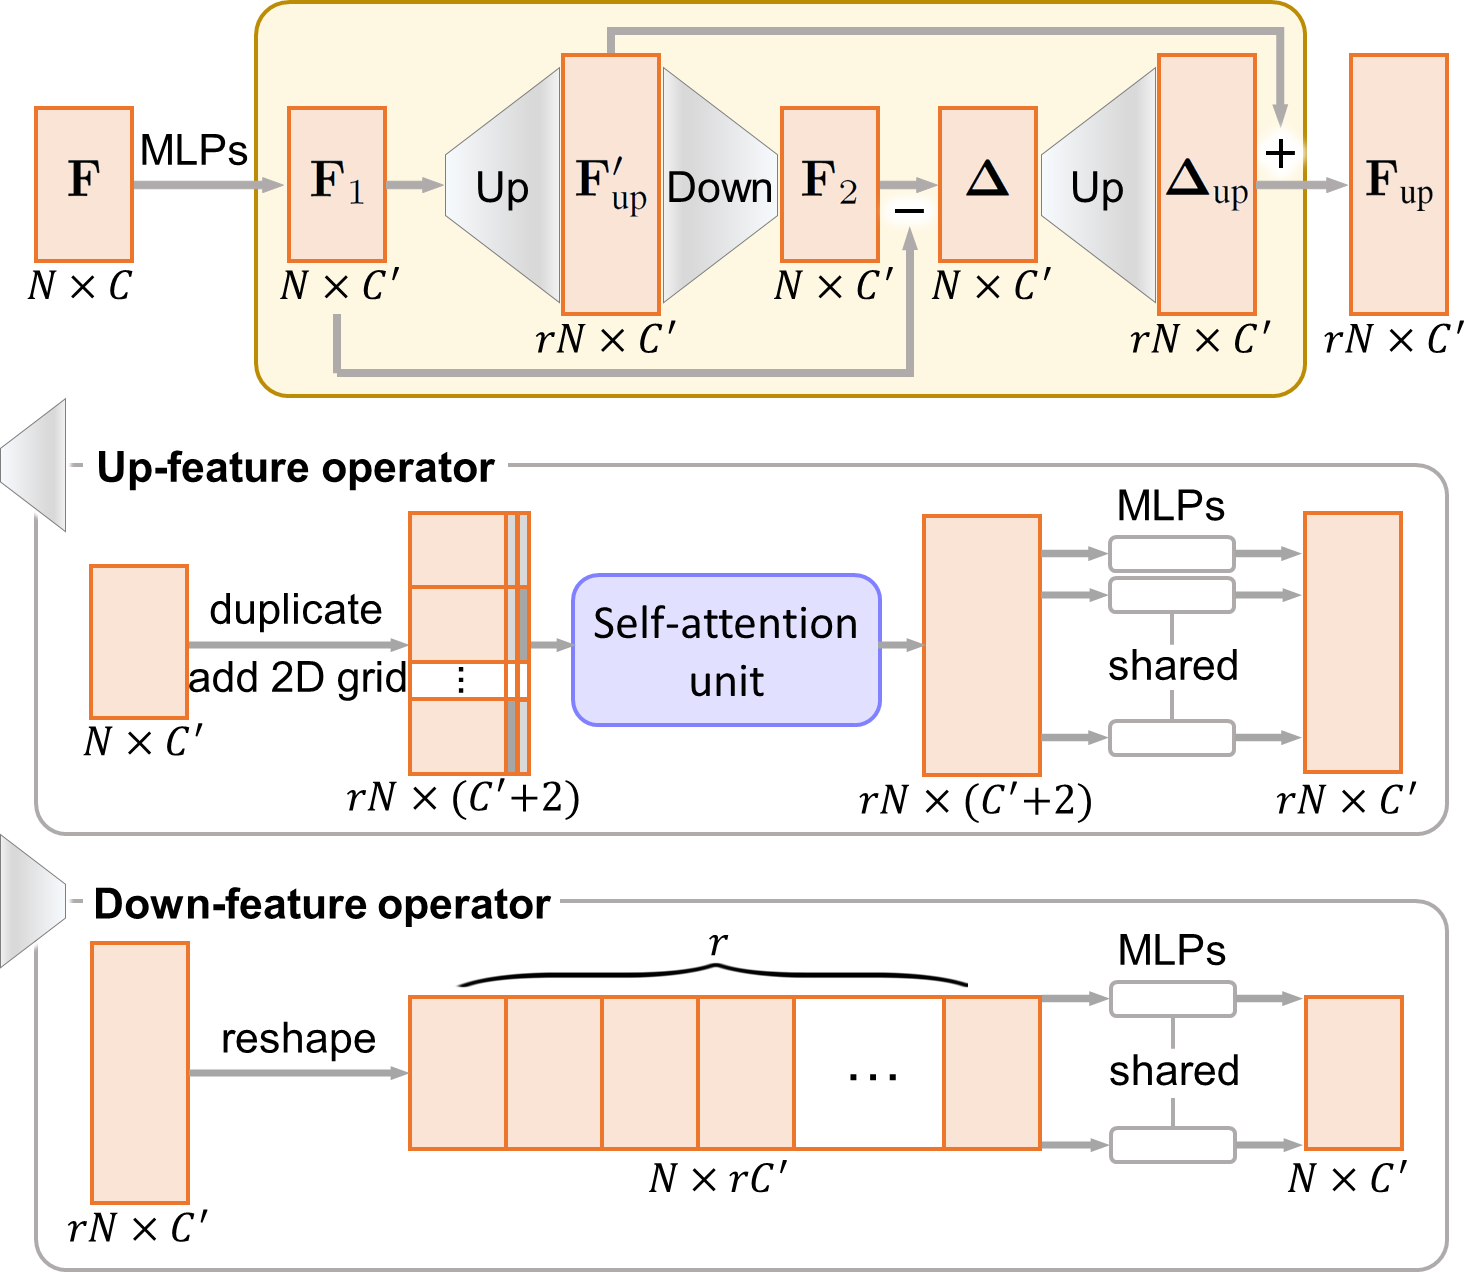
\includegraphics[width=0.98\linewidth]{block}
	\caption{The up-down-up expansion unit (top), up-feature operator (middle), and down-feature operator (bottom).}
	\label{fig:block}
	\vspace*{-2mm}
\end{figure}

%Different from~\cite{yu2018pu} and~\cite{yifan2018patch}
In this work, we construct an up-down-up expansion unit to expand the point features.
To do so, we first upsample the point features (after MLPs) to generate $\mathbf{F}_{\text{up}}^\prime$ and downsample it back (see Figure~\ref{fig:block} (top)); then, we compute the difference (denoted as $\Delta$) between the features before the upsampling and after the downsampling.
By also upsampling $\Delta$ to $\Delta_{\text{up}}$, we add $\Delta_{\text{up}}$ to $\mathbf{F}_{\text{up}}^\prime$ to self-correct the expanded features;
% to $\mathbf{F}_{\text{up}}$;
see again Figure~\ref{fig:block} (top) for the whole procedure.
Such a strategy not only avoids tedious multi-step training, but also facilitates the production of fine-grained features.
%, thus leading to better reconstructions.

%\phil{a bit straightforward, so I commented these:}
%Specifically, this unit consists of the following sequential steps:
%\begin{enumerate}
%	\item MLPs: $\mathbf{F}_1=f_{\text{mlp}}(\mathbf{F})$
%	\item feature up operation: $\mathbf{F}_{\text{up}}^\prime=f_{\text{up}}(\mathbf{F}_1)$,
%	\item feature down operation: $\mathbf{F}_2=f_{\text{down}}(\mathbf{F}_{\text{up}}^\prime)$,
%	\item residual: $\mathbf{\Delta}=\mathbf{F}_2-\mathbf{F}_1$,
%	\item residual up operation: $\mathbf{\Delta}_{\text{up}}=f_{\text{up}}(\mathbf{\Delta})$,
%	\item summation: $\mathbf{F}_{\text{up}}=\mathbf{F}_{\text{up}}^\prime+\mathbf{\Delta}_{\text{up}}$,
%\end{enumerate}
%Note that $f_{\text{mlp}}$ means the MLPs operation, $f_{\text{up}}$ and $f_{\text{down}}$ denote the feature up and down operations, respectively, and will be detailed later.

%From the above sequential steps we can see that, we organize this unit by alternating between upsampled and downsampled features.
%Compared with the feature expansion in one step, like PU-Net, our up-down-up expansion unit can be regarded as a self-correcting %procedure which feeds the upsampling error ($\mathbf{\Delta}$) to the sampling layer and corrects the solution by adding back the %upsampled error ($\mathbf{\Delta}_{\text{up}}$).
%Hence, this enables a more fine-grained expanded feature map, leading to better reconstruction results.
%\phil{it seems that this paragraph has no new contents/information compared to the paragraph before it... can you shorten it OR %remove it?}

%\if 0
%\begin{figure}[t]
%	\centering
%	\includegraphics[width=1.0\linewidth]{imgs/up_down}
%	\caption{The details of our up operation and down operation.}
%	\label{fig:up_down}
%\end{figure}
%\fi

Next, we discuss the up-feature and down-feature operators in the up-down-up expansion unit (see also Figure~\ref{fig:block}):

\para{Up-feature operator.} \
%The goal of the feature up operation is to
To upsample the point features $r$ times, we should increase the variations among the duplicated features.
This is equivalent to pushing the new points away from the input ones.
%
After we duplicate the input feature map (of $N$ feature vectors and $C'$ channels) $r$ times, we adopt the 2D grid mechanism in FoldingNet~\cite{yang2018foldingnet} to generate a unique 2D vector per feature-map copy, and append such vector to each point feature vector in the same feature-map copy; see Figure~\ref{fig:block} (middle).
%
Further, we use the self-attention unit (see Section~\ref{subsec:attention}) followed by a set of MLPs to produce the output upsampled features.

\para{Down-feature operator.} \
To downsample the expanded features, we reshape the features and then use a set of MLPs to regress the original features; see Figure~\ref{fig:block} (bottom).



%feature contents except for these values
%we first duplicate the whole feature map $r$ times.
%Then we generate a 2D grid with $r$ elements. For each element, we duplicate its coordinate $N$ times to form a $N \times 2 $ vector, and then append it to one of duplicated feature vectors; see Figure~\ref{fig:block} (middle). Note that we do not use the value of each element and we just use the coordinate.

%This mechanism is adopted from the code assignment mechanism in FoldingNet~\cite{yang2018foldingnet}, so that each copy of the duplicated feature vector has a 2D coordinate as an unique label. In this way, we can increase the feature variations before feeding the features to the self-attention unit and then the MLPs; see again Figure~\ref{fig:block} (middle). Moreover, to better blend the concatenated latent code, we employ a self-attention unit and then adopt a set of MLPs to generate the upsampled features.
%two values from a 2D grid attached to it like a label.

%Here, the coordinate is selected from a zero-centered $\sqrt{r} \times \sqrt{r}$ (equals to $r$) grid with side length $s=0.2$.
%By using bilinear interpolation between $[-s,s]$, we can obtain two values at each grid position.

% then append coordinates in a 2D grid to each of the $rN$ feature vectors; see Figure~\ref{fig:block} (middle). Here, the random values are generated by ... \phil{how are they created? need one or two sentences here to describe... but please write in a way that others can understrand}
%
%\phil{I really can't follow the details!!!!!!! E.g., what is $n_x$ and $n_y$? you must define every symbol! what is $s$? in what space? no one can really understand!!!}
%To upsample the features $r$ times, we should try to avoid producing new points close to the original points, similar to FoldingNet~\cite{yang2018foldingnet}, we adopt the idea of code assignment by appending a 2D grid to augment the internal representation variation; see Figure~\ref{fig:block} (middle).
%to each copy of the duplicated features
%Specifically, we first generate a zero-centered $n_x \times n_y$ (equals to $r$) grid with side length $s=0.2$.
%By using bilinear inerpolation between $[-s,s]$, we can obtain two values at each grid position.
%We then organize their coordinates into a $r \times 2$ matrix.
%At last, we duplicate each row of the matrix $N$ times and attach it to each copy of the duplicated features.
%Then we duplicate each row of the matrix $N$ times and concatenate it with each copy of the duplicated features.
%We generate the 2D grid by \phil{Please add some details about the grid values}.

%\phil{the word series has the meaning of successive... so, shall we use set instead?}

%
%The goal of the feature down operation is to recover the original feature map with $N \times C^\prime$ from the expanded feature map with $rN \times C^\prime$.
%The process is illustrated in the bottom row of Figure~\ref{fig:block}, where we first reshape the expanded features and then add MLPs to regress the original feature map.



%%%%%%%%%%%%%%%%%%%%%%%%%%%%%%%%%%%%%%%%%%%%%%%%%%%%%%%%%%%

\subsection{Self-attention Unit}
\label{subsec:attention}

\rh{To introduce long-range context dependencies to enhance feature integration after concatenation}, we adopt the self-attention unit~\cite{zhang2019self} in the generator (see Figure~\ref{fig:block} (middle)), as well as in the discriminator (see Figure~\ref{fig:framework} (bottom)).
%\rh{ We employed the self-attention idea ~\cite{zhang2019self} to introduce long-range context dependencies to improve the
%quality of the point features, rather than simply extracting
%per-point features individually.}
%Compared with the basic MLPs, it helps to better combine and integrate features after concatenation.
%
Figure~\ref{fig:attention} presents its architecture.
%
Specifically, we transform the input features into $\mathbf{G}$ and $\mathbf{H}$ via two separate MLPs, and then generate the attention weights $\mathbf{W}$ from $\mathbf{G}$ and $\mathbf{H}$ by
%
\begin{equation}
\mathbf{W} = f_{\text{softmax}}(\mathbf{G}^T \mathbf{H}) \ ,
\end{equation}
%
where $f_{\text{softmax}}$ denotes the softmax function.
After that, we obtain the weighted features $\mathbf{W}^T\mathbf{K}$, where $\mathbf{K}$ is the set of features extracted from the input via another MLP.
Lastly, we generate the output features, which is the sum of the input features and the weighted features.


%\phil{why need MLP before K? How if we remove the bottom-most MLP and K in the attention diagram and multiply W directly with the input features to produce the output features?}
%
%see the ablation study in Section~\ref{subsec:ablation}.
%see an experiment in Section~\ref{sec:experiment}.
%
%This network unit is employed inside both the generator and discriminator networks; see the middle row in Figure~\ref{fig:block} and the bottom row in Figure~\ref{fig:framework}, respectively.

%As we have mentioned above, we add a self-attention unit after the feature concatenation operation inside the feature up operation and the discriminator, respectively.
%Compared with the simple MLPs, this unit can better mix and blend the concatenated features, so that the subsequently extracted features are more expressive.
%Figure~\ref{fig:attention} present the details of the self-attention unit.

%Specifically, the input features are first transformed into two feature space $\mathbf{G}$, $\mathbf{H}$ via MLPs, and the %attention weights $\mathbf{W}$ are calculated by:
%\begin{equation}
%	\mathbf{W} = f_{\text{softmax}}(\mathbf{G}^T \mathbf{H}),
%\end{equation}
%where $f_{\text{softmax}}$ denotes the softmax function.
%Then the output of this attention layer is $\mathbf{W}^T\mathbf{K}$, where $\mathbf{K}$ is the extracted feature map from the %input features via MLPs.

\begin{figure}[!t]
	\centering
	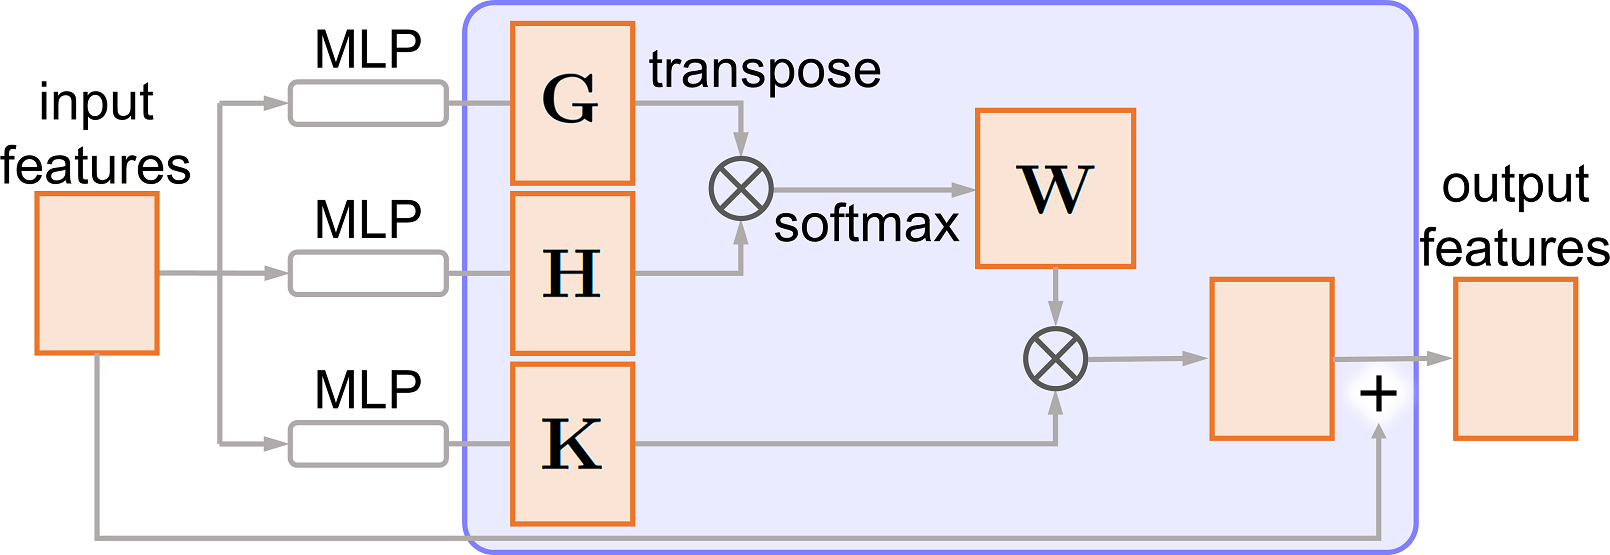
\includegraphics[width=0.75\linewidth]{attention}
	\caption{Illustration of the self-attention unit.}
	\label{fig:attention}
	\vspace*{-2mm}
\end{figure}



%%%%%%%%%%%%%%%%%%%%%%%%%%%%%%%%%%%%%%%%%%%%%%%%%%%%%%%%%%%

\subsection{Patch-based End-to-end Training}
\label{subsec:training}

\subsubsection{Training data preparation}
\label{subsubsec:train_data}

%\phil{after understanding sec 3.5 more, I think we miss an important subsection here to talk about the training and testing dataset, how we produce $\mathbf{P}$ and $\mathbf{\hat{Q}}$, as well as anything that should be done BEFORE the network training}

%\phil{this subsection is to prepare for the data and patches for defining the losses!!!!}

%\phil{So, move Sec 4.1 here and MODIFY... read then modify.. reaad then modify, repeat this at least 3-5 times}

\begin{figure}
	\centering
	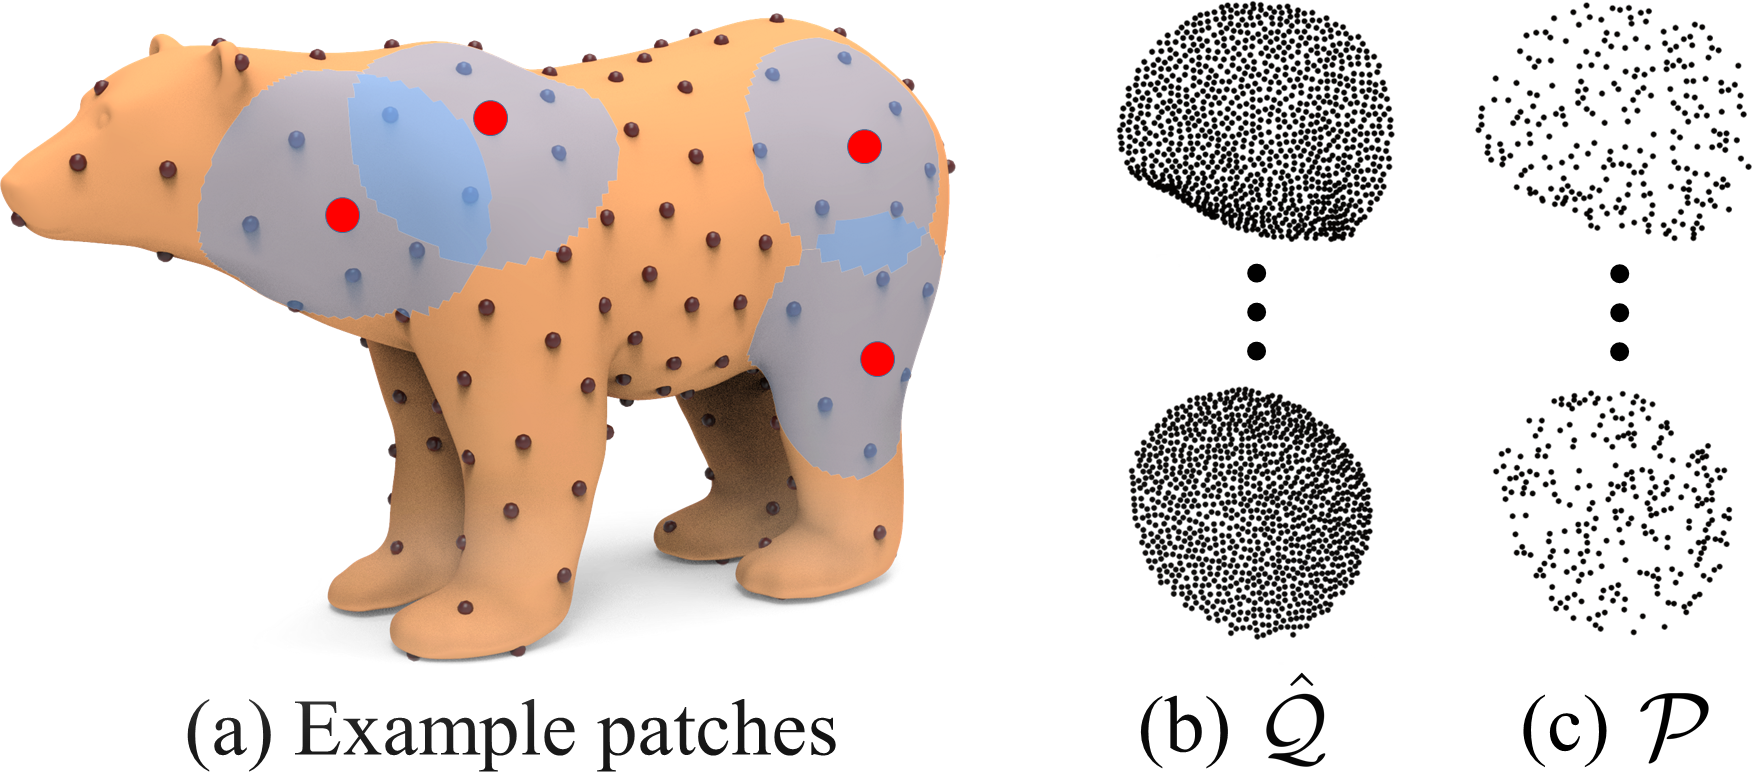
\includegraphics[width=0.9\linewidth]{patch_segment}
	\caption{(a) Seed points (black dots) and patches (blue disks) on a 3D mesh in training data.
(b) \& (c) Example $\mathcal{\hat{Q}}$ and $\mathcal{P}$ on patches.}
%	\caption{Illustration of the training data preparation: (a) we select 200 seed points (black dots) on the object surface and grow a patch (blue circle) at each seed (red dots); (b) we generate a target point set
%$\mathcal{\hat{Q}}$ with $rN$ points on the patch; (c) we generate the network input $\mathcal{P}$ by randomly selecting $N$ points on-the-fly from $\mathcal{\hat{Q}}$.}
	\label{fig:patch_segment}
	\vspace*{-2mm}
\end{figure}

We trained our network to upsample local groups of points over patches on object surface.
%\phil{a small figure to show one or two 3D meshes and a few sample input patches (P) on them?}
%
Specifically, for each 3D mesh (normalized in a unit sphere) in training set (see Section~\ref{subsec:dataset}), we use randomly
%farthest sampling to
find 200 seed positions on each mesh surface, geodesically grow a patch from each seed (each patch occupies $\sim$5\% of the object surface), and then normalize each patch within a unit sphere; see Figure~\ref{fig:patch_segment}(a).
%
On each patch, we further use Poisson disk sampling~\cite{corsini2012efficient} to generate $\mathcal{\hat{Q}}$, which is a target point set of $rN$ points on the patch.
During the training, we generate the network input $\mathcal{P}$ by randomly selecting $N$ points on-the-fly from $\mathcal{\hat{Q}}$.

%%%%%%%%%%%%%%%%%%%%%%%%%%%%%%%%%%%%%%%%%%%%%%%%%%%%%%%%%%%
\subsubsection{Loss functions}
\label{subsubsec:loss}


We now present the compound loss designed for training PU-GAN in an end-to-end fashion.

%In this subsection, we illustrate loss functions that are employed to train our PU-GAN in an end-to-end fashion, which consists of an \emph{adversarial loss}, a \emph{uniform loss} and a \emph{reconstruction loss}.



%%%%%%%%%%%%%%%%%%%%%%%%%%%%%%%%%%%%%%%%%%%%%%

\para{Adversarial loss.} \
%To stabilize our model training procedure and have a high convergence rate,
To train the generator network $G$ and discriminator network $D$ in an adversarial manner, we use the least-squared loss~\cite{mao2017least} as our adversarial loss:
%
\begin{eqnarray}
\mathcal{L}_{\text{gan}}(G)&=&\frac{1}{2}[D(\mathcal{Q})-1]^2 \\
\text{and} \ \
\mathcal{L}_{\text{gan}}(D)&=&\frac{1}{2}[D(\mathcal{Q})^2 + (D(\mathcal{\hat{Q}})-1)^2],
\end{eqnarray}
%
where
%$\mathcal{Q}$ is the generator output;
%$\mathcal{\hat{Q}}$ is the target point set;
%and
$D(\mathcal{Q})$ is the confidence value predicted by $D$ from generator output $\mathcal{Q}$.
%
During the network training, $G$ aims to generate $\mathcal{Q}$ to fool $D$ by minimizing $\mathcal{L}_{\text{gan}}(G)$, while $D$ aims to minimize $\mathcal{L}_{\text{gan}}(D)$ to learn to distinguish $\mathcal{Q}$ from $\mathcal{\hat{Q}}$.
%
%In the training process, $\mathcal{Q}$ and $\mathcal{\hat{Q}}$ need not be paired, and we produce $\mathcal{\hat{Q}}$ by Poisson disk sampling on the underlying object surface.
%\phil{the last sentence here better goes to the new Sec 3.5}
%In the testing process, only the well-trained generator needs to be utilized to reconstruct a point cloud from a sparse input.
%Compared with the traditional logarithmic loss function, we empirically found that the least-squared loss helps produce higher-quality results than to converge the generated data distribution to the decision boundary\cite{zhu2017unpaired},



%%%%%%%%%%%%%%%%%%%%%%%%%%%%%%%%%%%%%%%%%%%%%%

\para{Uniform loss.} \
The problem of learning to generate point sets in 3D is complex with an immense space for exploration during the network training.
Particularly, we aim for uniform distributions; using the adversarial loss alone is hard for the network to converge well.
%making it hard for the network to converge well with the adversarial loss alone.
%making it hard for the network to converge well .
Thus, we formulate a uniform loss to evaluate $\mathcal{Q}$ from the generator, aiming to improve the generative ability of the generator.
% and promote the discriminator to learn more latent patterns.
% from the target distribution.
%
%Only relying on the adversarial loss is not powerful enough, since it is a random and complex procedure to encourage the generator to converge and generate a uniform distribution during training process.
%Hence, to further stabilize and accelerate the convergence of the GAN framework, we formulate a uniform loss in the generator to enhance the distribution uniformity in the generated points, thus promoting the discriminator to discover more latent patterns from the target distribution.

To evaluate a point set's uniformity, the NUC metric in PU-Net~\cite{yu2018pu} crops equal-sized disks on the object surface and counts the number of points in the disks.
So, the metric neglects the local clutter of points.
Figure~\ref{fig:uniformity} shows three patches of points with very different point distributions; since they contain the same number of points, the NUC metric cannot distinguish their distribution uniformity.
%allowing us to evaluate the point distribution uniformity from small local scales to larger global scales.
%the points are whether the points are locally too close to their neighbors.
%since they have the same number of points, their NUC values are the same.
%the three point sets have the same point number, but the distributions are totally different.
%\phil{revise this sentence after Fig.5 is fixed}

\begin{figure}[t]
	\centering
	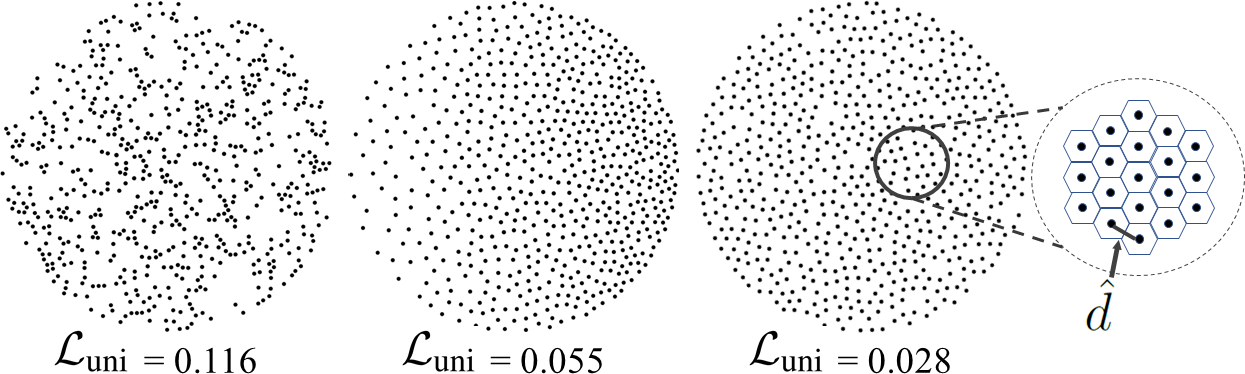
\includegraphics[width=1.0\linewidth]{uniform_example}
	\caption{Example point sets with same number of points (625) but different point distribution patterns; $\mathcal{L_{\text{uni}}}$ is computed with $p$$=$$1\%$.}
%We set $p=1\%$ for uniformity calculation.}
	\label{fig:uniformity}
	\vspace*{-2mm}
\end{figure}

Our method evaluates $\mathcal{Q}$ (a patch of $rN$ points) during the network training by first using the farthest sampling to pick $M$ seed points in $\mathcal{Q}$ and using a ball query of radius $r_d$ to crop a point subset (denoted as $S_j$, $j=1..M$) in $\mathcal{Q}$ at each seed.
Here, we use a small $r_d$, so $S_j$ roughly lies on a small local disk of area $\pi r_d^2$ on the underlying surface.
%
On the other hand, since we form patches by geodesics and normalize them in a unit sphere, patch area is $\sim$$\pi 1^2$.
%generated $\mathcal{Q}$ could be roughly unfolded as a 2D circle with the radius of 1.
%Considering that each training patch $\mathcal{Q}$ is geodesically segmented on the object surface and is normalized within a canonical sphere, each patch thus could be unfolded as a 2D circle with the radius of 1.
So, the expected percentage of points in $S_j$ (denoted as $p$) is $\pi r_d^2 / \pi 1^2 = r_d^2$, and the expected number of points in $S_j$ (denoted as $\hat{n}$) is $rNp$.
%
Hence, we follow the chi-squared model to measure the deviation of $|S_j|$ from $\hat{n}$, and define
%
\begin{equation}
U_{\text{imbalance}}(S_j) = \frac{(|S_j|-\hat{n})^2}{\hat{n}} \ .
\end{equation}

To account for local point clutter, for each point in $S_j$, we find its distance to the nearest neighbor, denoted as $d_{j,k}$ for the $k$-th point in $S_j$.
If $S_j$ has a uniform distribution, the expected point-to-neighbor distance $\hat{d}$ should be roughly $\sqrt{\frac{2\pi r_d^2}{|S_j| \sqrt{3}}}$, which is derived based on the assumption that $S_j$ is flat and neighboring points are hexagonal; see Figure~\ref{fig:uniformity} (right) for an illustration and supplemental material for the derivation.
%
Again, we follow the chi-squared model to measure the deviation of $d_{j,k}$ from $\hat{d}$, and define
%
\begin{equation}
U_{\text{clutter}}(S_j) = \sum_{k=1}^{|S_j|} \frac{(d_{j,k}-\hat{d})^2}{\hat{d}} \ .
\end{equation}
%where $d_{j,k}$ represents the distance between the $k$-th point inside the $j$-th disk and its nearest neighbor.

Here, $U_{\text{clutter}}$ accounts for the local distribution uniformity, while $U_{\text{imbalance}}$ accounts for the nonlocal uniformity to encourage better point coverage.
Putting them together, we formulate the uniform loss as
%
\vspace*{-1.5mm}
\begin{equation}
\label{eq:uniform}
\mathcal{L_{\text{uni}}} = \sum_{j=1}^{M}U_{\text{imbalance}}(S_j) \cdot U_{\text{clutter}}(S_j) \ .
\vspace*{-1mm}
\end{equation}
%
Figure~\ref{fig:uniformity} shows three example point sets with the same number of points but different point distribution patterns.
Using $\mathcal{L_{\text{uni}}}$, we can distinguish the point uniformity among them.
%we can see that, our proposed uniform loss is not only sensitive to local uniformity, but also the global uniformity; see particularly the middle point set.
%


%Then, the area percentage (denoted as $p$) of the local disk over the patch described by $\mathcal{Q}$ can be approximated by $\pi r_d^2/\pi 1^2=r_d^2$.
%with the assumption that the disk is regarded as a 2D circle since it is commonly small enough.
%
%
%We then grow a small disk centered around each seed by using the query ball with the radius of $r_d$.
%Considering that we geodesically \phil{it is wrong to say geodesically here in the training process, right?} crop and normalize each training patch \phil{what exactly is a patch? in methodology, writing should be precise and specific... what is a patch? $\mathcal{Q}$? Never use a term that hasn't been defined clearly in the methodology section}
%within a sphere with radius one, thus the area percentage (denoted as $p$) of the disk over the patch can be calculated \phil{approximated, right?  Another important thing in writing is PRECISION!!!!} by $\pi r_d^2/\pi 1^2=r_d^2$, assuming \phil{..., for small $r_d$.}
%where we approximate both the disk and the patch as 2D circles by considering that the disk is small enough and the patch is geodesically cropped, thus could be unfolded as 2D circles with very few errors.
%\phil{why 1 in the equation? there should be some reasons that you need to explain, right?}
%In our implementation, %instead of a single fixed disk area percentage $p$,
%we obtain multiple small disks around each seed with varying $p$ (\ie, 0.4\%, 0.6\%, 0.8\%, 1.0\%, and 1.2\%).
%For each area percentage $p$, we define $n_j$ as the point number inside the $j$-th disk and $\hat{n}$ as the expected point number for each disk.
%Then, for the $j$-th disk with the number of points as $n_j$, on the one hand,
%If the generated $rN$ points are uniformly-distributed on the patch, the expected point number $\hat{n}$ of each disk can be approximated by $rN \times p$.
%Here, we employ the chi-squared test to measure the imbalance between $n_j$ and $\hat{n}$ given the $j$-th disk, which is denoted as:
%
%\begin{equation}
%	U_{\text{imbalance}}(j) = \frac{(n_j-\hat{n})^2}{\hat{n}}.
%\end{equation}

%On the other hand, if points are uniformly-distributed inside the $j$-th disk of the radius $r_d$ , the expected adjacent point distance $\hat{d}$ can be approximated by $\sqrt{\frac{2\pi r_d^2}{n_j \times \sqrt{3}}}$
%\phil{you MUST prepare a supp. section to derive this number step by step... do it ASAP to make sure that this formulae is correct... I doubt}
%with the assumption that we uniformly split the disk using hexagons of the same size; see the illustration on the rightmost of Figure~\ref{fig:uniformity}.
%Please refer to the supplementary material for the detailed derivation of $\hat{d}$.
%Thus, we formulate the following term to account for the cohesion:
%\begin{equation}
%U_{\text{cohesion}}(j) = \sum_{k=1}^{n_j} \frac{(d_{j,k}-\hat{d})^2}{\hat{d}},
%\end{equation}
%where $d_{j,k}$ represents the distance between the $k$-th point inside the $j$-th disk and its nearest neighbor.

%For the sake of computational efficiency, we design a uniform loss based on a simplified version of the uniformity metric. First, we extract a series of partitions defined as a neighborhood ball in the underlying Euclidean space. To evenly cover the whole surface, the centroids are selected among generated point set by a farthest point sampling (FPS) algorithm. Within our assumption, the normalized patch-based inputs can be regarded as a round surface with a radius 1. Given the size of each neighborhood ball, we can obtain the expected inside number of points $\hat{N}$. In that case, we directly query $\hat{N}$ points for each centroid given a query radius $r$. We will duplicate the centroid point if inside point number is less than $\hat{N}$ and select the nearest $\hat{N}$ point if there are too many point in one ball(whole process is implemented by the ball query ~\cite{qi2017pointnet++}). Finally, the uniform loss is formulated by:

%\begin{equation}
%\mathcal{L_{\text{uni}}} &=& \sum_{D}^{i=0}\sum_{\hat{N}}^{j=0}\left(\frac{(d_{ij}-\hat{d_i})^2}{\hat{d_i}}\right)\\
%\hat{d_i}&=&\sqrt{\frac{2\pi r^2}{\sqrt{3}}}
%\end{equation}
%where $d_{ij}$ represents the distance between $jth$ point and its nearest neighbour and $\hat{d_i}$ is the corresponding expected distance and it will be the same for all balls given a fixed radius.



%%%%%%%%%%%%%%%%%%%%%%%%%%%%%%%%%%%%%%%%%%%%%%

\para{Reconstruction loss.} \
Both the adversarial and uniform losses do not encourage the generated points to lie on the target surface.
Thus, we include a reconstruction loss using the Earth Mover's distance (EMD)~\cite{fan2016point}:
%to emphasize the geometric consistency between the predicted point set and the sampled point set on the surface:
%
\vspace*{-1.5mm}
\begin{equation}
	\mathcal{L_{\text{rec}}} = \min_{\phi:\mathcal{Q}\rightarrow \mathcal{\hat{Q}}} \sum_{q_i\in \mathcal{Q}} \|q_i-\phi(q_i)\|_2,
	\vspace*{-1mm}
\end{equation}
%
where %$\mathcal{\tilde{Q}}$ is a sampled patch of points co-located with $\mathcal{Q}$, simply for representing the underlying object surface, and
$\phi:\mathcal{Q}\rightarrow \mathcal{\hat{Q}}$ is the bijection mapping.



%%%%%%%%%%%%%%%%%%%%%%%%%%%%%%%%%%%%%%%%%%%%%%

\para{Compound loss.} \
Overall, we train PU-GAN end-to-end by minimizing $\mathcal{L}_G$ for generator and  $\mathcal{L}_D$ for discriminator:
\begin{eqnarray}
\label{eq:compound}
	\mathcal{L}_G&=& \lambda_{\text{gan}}\mathcal{L_{\text{gan}}}(G) +\lambda_{\text{rec}}\mathcal{L_{\text{rec}}} + \lambda_{\text{uni}}\mathcal{L_{\text{uni}}}, \\
	\text{and} \ \
    \mathcal{L}_D&=&\mathcal{L}_{\text{gan}}(D),
\end{eqnarray}
where $\lambda_{\text{gan}}$, $\lambda_{\text{rec}}$, and $\lambda_{\text{uni}}$ are weights.
%to balance the relative importance of each loss term.
During the training process, $G$ and $D$ are optimized alternatively.

%why we do not sample centroids on the uniform sample, cause if do so, at the begining, the unform will take a prominent position with a non-uniform outputs, however, we need to be steady to train the nerwork


\section{Experiments}
\label{sec:experiment}

%In this section, we compare the proposed PU-GAN quantitatively and qualitatively with state-of-the-art point upsampling methods, and evaluate various aspects of our model. Please refer to the supplementary for extended experiments. Upon publication, we will release the full training and test data set, as well as the trained network and source code.
%for further implementation details

\begin{figure*}[t]
	\centering
	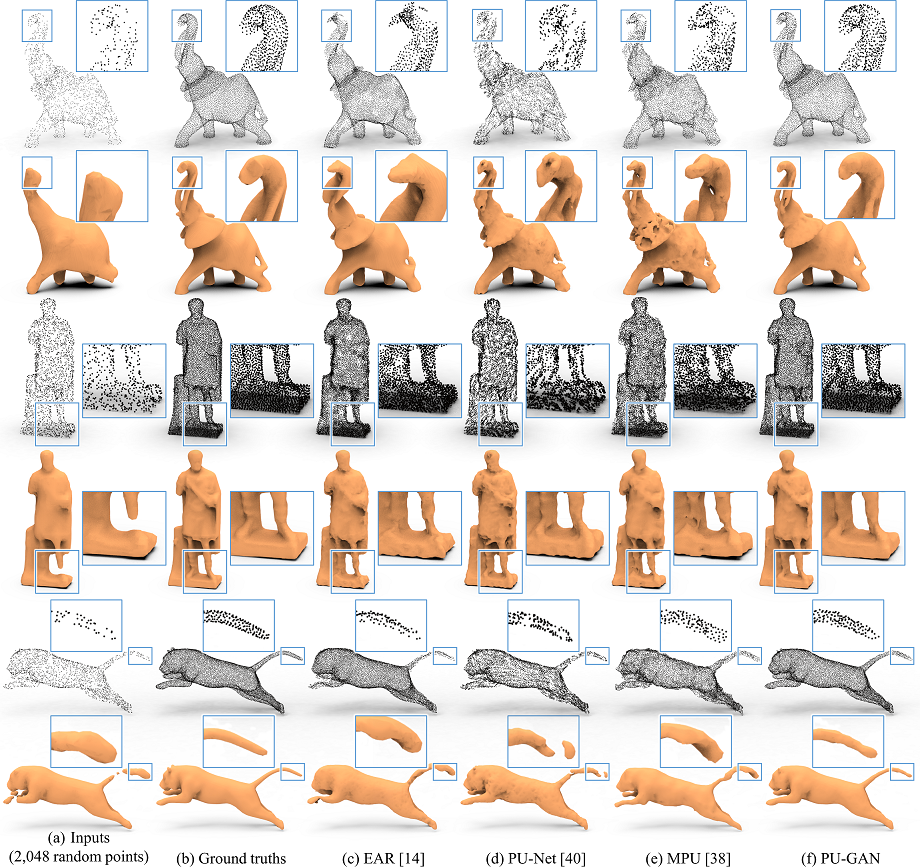
\includegraphics[width=0.99\linewidth]{visualComparison}
	\caption{Comparing point set upsampling (x4) and surface reconstruction results produced with different methods (c-f) from inputs (a).}
%	\caption{Comparing the point set upsampling results and the mesh reconstruction results produced using different methods (c-f) from inputs (a) with 2,048 non-uniform points.}
	\label{fig:visualComparison}
	\vspace*{-2mm}
\end{figure*}

%%%%%%%%%%%%%%%%%%%%%%%%%%%%%%%%%%%%%%%%%%%%%%%%%%%%%%%%%%%

\begin{figure*}[t]
	\centering
	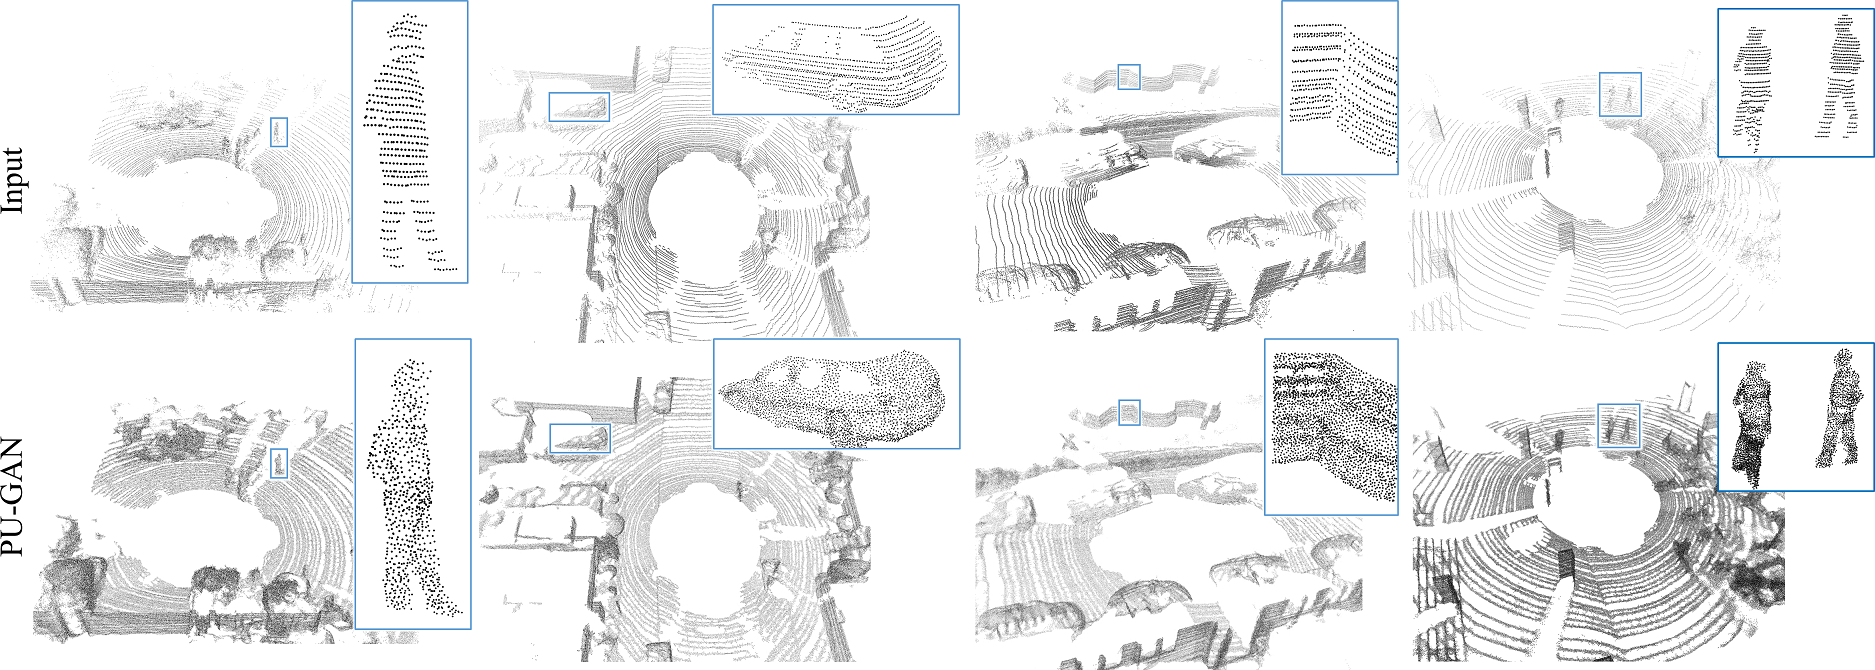
\includegraphics[width=1.0\linewidth]{realscan}
	\caption{Using PU-GAN to upsample real-scanned point cloud data acquired by LiDAR.}
	\label{fig:realscan}
	\vspace*{-2mm}
\end{figure*}



%%%%%%%%%%%%%%%%%%%%%%%%%%%%%%%%%%%%%%%%%%%%%%%%%%%%%%%%%%%



%%%%%%%%%%%%%%%%%%%%%%%%%%%%%%%%%%%%%%%%%%%%%%%%%%%%%%%%%%%

\subsection{Datasets and Implementation Details}
\label{subsec:dataset}
We collected 147 3D models from the released datasets of PU-Net~\cite{yu2018pu} and MPU~\cite{yifan2018patch}, as well as from the Visionair repository~\cite{visionair}, covering a rich variety of objects, ranging from simple and smooth models (\eg, Icosahedron) to complex and high-detailed objects (\eg, Statue); see the supplemental material for all of them.
Among them, we randomly select 120 models for training and use the rest for testing.
%We totally collect 147 models from the released datasets of PU-Net~\cite{yu2018pu} and MPU~\cite{yifan2018patch}, as well as the Visionair repository~\cite{visionair}, covering a variety of objects ranging from smooth and simple structures (\eg, Icosahedron) to complex and high-detailed objects (\eg, Statue); see the supplemental material for all the models.
%Among these models, we randomly select 120 for training and the rest 27 models for testing.

%On each patch, we employ Poisson disk sampling~\cite{corsini2012efficient} algorithm to generate 1,024 points as target uniform samples and then randomly select $N=256$ points on-the-fly from the sampled 1,024 points as inputs and feed them into the network for training.
%By default, the upsampling rate $r=4$.

%In the testing phase, we first use Poisson disk sampling to sample 8,192 points as ground truth on the object surface and then randomly select 2,048 points for testing.
%Note that, following MPU~\cite{yifan2018patch}, we also adopt the patch-based testing strategy.
%Specifically, we apply farthest sampling to select 24 seeds from the 2,048 points, and then grow a point subset at each seed with 256 points.
%We feed these point subsets into the generator for upsampling, and then combine the upsampled points together, apply the farthest sampling to get the final upsampled point cloud with 8,192 points.



%%%%%%%%%%%%%%%%%%%%%%%%%%%%%%%%%%%%%%%%%%%%%%%%%%%%%%%%%%%

%\subsection{Implementation Details}
%\label{subsec:implementation}

In the training phase, we cropped 200 patches per training model (see Section~\ref{subsubsec:train_data}) and produced $24,000$ patches in total.
By default, we set $N=256$, $r=4$, and $M=50$.
Moreover, for the uniform loss, we cropped one set of $S_j$ with radius $r_d=\sqrt{p}$ for each $p \in$ \{ 0.4\%, 0.6\%, 0.8\%, 1.0\%, 1.2\% \}, compute Eq.~\eqref{eq:uniform} five times for each set, and then sum up the results as the $\mathcal{L_{\text{uni}}}$ term in Eq.~\eqref{eq:compound}.

To avoid overfitting in training, we augment the network inputs by random rotation, scaling, and point perturbation with Gaussian noise.
%To calculate $\mathcal{L_{\text{uni}}}$ during training, we set the number of disks $M=50$.
We trained the network for 100 epochs using the Adam algorithm~\cite{kingma2014adam} with a two time-scale update rule (TTUR)~\cite{heusel2017gans}.
We set the learning rates of generator and discriminator as 0.001 and 0.0001, respectively; after 50k iterations, we gradually reduce both rates by a decay rate of 0.7 per 50k iterations until $10^{-6}$.
The batch size is 28, and $\lambda_{\text{rec}}$, $\lambda_{\text{uni}}$, and $\lambda_{\text{gan}}$ are empirically set as 100, 10, and 0.5, respectively.
We implemented our network using TensorFlow and trained it on NVidia Titan Xp GPU.

During the testing, given a point set, we follow the patch-based strategies in MPU~\cite{yifan2018patch} and EC-Net~\cite{yu2018ec} to use the farthest sampling to pick seeds and extract a local patch of $N$ points per seed.
Then, we feed the patches to the generator and combine the upsampled results as the final output.



%%%%%%%%%%%%%%%%%%%%%%%%%%%%%%%%%%%%%%%%%%%%%%%%%%%%%%%%%%%

\subsection{Evaluation Metrics}
\label{subsec:evaluation}
We employ four evaluation metrics: (i) uniformity using $\mathcal{L_{\text{uni}}}$ in Eq.~\eqref{eq:uniform}, (ii) point-to-surface (P2F) distance using the testing models, (iii) Chamfer distance (CD), and (iv) Hausdorff distance (HD)~\cite{berger2013benchmark}.
For quantitative evaluation, we use Poisson disk sampling to sample 8,192 points as the ground truth (\eg, see Figure~\ref{fig:visualComparison}(b)) on each of the testing models, and randomly select 2,048 points as testing input.
To evaluate the uniformity of the test results (using Eq.~\eqref{eq:uniform}), we randomly pick $M=1,000$ seeds on each result, and instead of using ball query to crop $S_j$, we use the actual mesh (testing model) to geodesically find $S_j$ at each seed of different $p$ for higher-quality evaluation.
The lower the metric values are, the better the upsampling results are.



%%%%%%%%%%%%%%%%%%%%%%%%%%%%%%%%%%%%%%%%%%%%%%%%%%%%%%%%%%%

\subsection{Qualitative and Quantitative Comparisons}
\label{subsec:comparison}

%\para{Comparison with state-of-the-arts.} \
We qualitatively and quantitatively compared PU-GAN with three state-of-the-art point set upsampling methods: EAR~\cite{huang2013edge}, PU-Net~\cite{yu2018pu}, and MPU~\cite{yifan2018patch}.
%Without additional surface and edge information, EC-Net\cite{yu2018ec} will degenerate into PU-Net.
For EAR, we employed the released demo code and generated the best results by exhaustively fine-tuning every associated parameter.
For PU-Net and MPU, we used their public code and retrained their networks using our training data.

Table~\ref{tab:quanComparison} shows the quantitative comparison results.
Our PU-GAN achieves the lowest values consistently for all the evaluation metrics.
Particularly, the uniformity of our results stays the lowest for all different $p$, indicating that the points generated by PU-GAN are much more uniform than those produced by others over varying scales.

Besides quantitative results, we show point set upsampling and surface reconstruction (using~\cite{kazhdan2013screened}) results for various models in Figure~\ref{fig:visualComparison}.
%The input point set has 2,048 non-uniform points and we upsample 4$\times$ for each approach.
%We reconstruct the surface from the point set by using the screened Poisson reconstruction algorithm~\cite{kazhdan2013screened}.
%Note that all the testing objects are different from the training objects.
Comparing the results produced by (f) our method and by (c-e) others, against (b) the ground truth points that are uniformly-sampled on the original testing models, we can see that other methods tend to produce more noisy and nonuniform point sets, thus leading to more artifacts in the reconstructed surfaces.
See, particularly, the blown-up views, showing that PU-GAN can produce more fine-grained details in the upsampled results,~\eg, elephant's nose (top) and tiger's tail (bottom).
%Hence, the reconstructed meshes by our PU-GAN are the closest to the ground truths.
More comparison results can be found in the supplemental material.

%For non-uniform consideration, we set a small $neighborhood \;  number = 10$ for PCA normal estimation\cite{hoppe1992surface} and $depth = 8$ for screened Possion reconstruction\cite{kazhdan2013screened}. As shown in Figure \ref{fig:visualComparison}, EAR maintains the upsampled points along the surface, but struggles with these regions of large gap. The non-uniform inputs have a huge negative impact on the performance of PU-Net, which tends to generate points around the original inputs. Instead of directly upsampling with 4 times, MPU can take advantage of all the intermediate multiples of data with a progressive training strategy. Based on that, MPU enables to fill more points in those non-contiguous areas but is difficult to produce clean and more well defined outputs. In comparison, our method is superior to all these methods quantitatively by a large margin. Qualitatively, our generated results are more uniform, less noisy and restore the underlying geometry.



%%%%%%%%%%%%%%%%%%%%%%%%%%%%%%%%%%%%%%%%%%%%%%%%%%%%%%%%%%%

\subsection{Upsampling Real-scanned Data}

Figure~\ref{fig:realscan} shows upsampling results on LiDAR point clouds (downloaded from KITTI dataset~\cite{geiger2013vision}) produced by PU-GAN.
From the first row, we can see the sparsity and non-uniformity of the inputs.
%Hence, it is quite challenging to upsample these points without any additional prior knowledge.\phil{hard to without prior knowledge... since the network also learns from the training set}
%Even under such case,
Our PU-GAN can still fill some holes and output more uniform points in the results; please see the supplemental material for more results.



\begin{table}[!t]
\centering
\caption{Quantitative comparisons with the state-of-the-arts.}
\label{tab:quanComparison}
\resizebox{\linewidth}{!}{
	\begin{tabular}{@{\hspace{1mm}}c@{\hspace{1mm}}||@{\hspace{1mm}}c@{\hspace{3mm}}c@{\hspace{3mm}}c@{\hspace{3mm}}c@{\hspace{3mm}}c@{\hspace{1mm}}|@{\hspace{0.2mm}}c@{\hspace{1mm}}|@{\hspace{1mm}}c@{\hspace{1mm}}|@{\hspace{1mm}}c@{\hspace{1mm}}} \toprule[1pt]
	\multirow{2}*{Methods} & \multicolumn{5}{@{\hspace{1mm}}c@{\hspace{1mm}}|@{\hspace{0.2mm}}}{Uniformity for different $p$ ($10^{-3}$)} & P2F & CD & HD \\ \cline{2-6}
	& 0.4\% & 0.6\% & 0.8\% & 1.0\% & 1.2\% & ($10^{-3}$) & ($10^{-3}$) & ($10^{-3}$)\\ \hline \hline
	EAR~\cite{huang2013edge}  &  16.84  & 20.27  & 23.98  &  26.15  & 29.18   & 5.82 & 0.52  & 7.37   \\
	PU-Net~\cite{yu2018pu} &  29.74  & 31.33  & 33.86  & 36.94   & 40.43 & 6.84 & 0.72  & 8.94   \\
	MPU~\cite{yifan2018patch} & 7.51  & 7.41  & 8.35  & 9.62   & 11.13  & 3.96 & 0.49  & 6.11   \\ \hline
	PU-GAN & \textbf{3.38} & \textbf{3.49}  & \textbf{3.44}  & \textbf{3.91}  & \textbf{4.64} & \textbf{2.33} & \textbf{0.28}  & \textbf{4.64}    \\ \bottomrule[1pt]
	\end{tabular}}
	%\vspace*{-2mm}
\end{table}

\begin{table}[t]
	\centering
	\caption{Quantitative comparisons:
		removing each specific component from the full PU-GAN pipeline (top five rows) vs. baseline GAN model (6-th row) vs. full PU-GAN pipeline (last row).}
	%	\caption{The upsampling results in terms of each evaluation metric when removing different component individually compared to our full pipeline, as well as the baseline results.}
	\label{tab:ablationStudy}
	\resizebox{\linewidth}{!}{
		\begin{tabular}{@{\hspace{1mm}}c@{\hspace{1mm}}||@{\hspace{1mm}}c@{\hspace{3mm}}c@{\hspace{3mm}}c@{\hspace{3mm}}c@{\hspace{3mm}}c@{\hspace{1mm}}|@{\hspace{0.2mm}}c@{\hspace{1mm}}|@{\hspace{1mm}}c@{\hspace{1mm}}|@{\hspace{1mm}}c@{\hspace{1mm}}} \toprule[1pt]
			\multirow{2}*{} & \multicolumn{5}{@{\hspace{1mm}}c@{\hspace{1mm}}|@{\hspace{0.2mm}}}{Uniformity for different $p$ ($10^{-3}$)} & P2F & CD & HD \\ \cline{2-6}
			& 0.4\% & 0.6\% & 0.8\% & 1.0\% & 1.2\% & ($10^{-3}$) & ($10^{-3}$) & ($10^{-3}$)\\ \hline \hline
			Discriminator       &  7.02  & 7.31  & 8.36  &  9.70  & 11.17  & 4.61 & 0.57  & 7.25  \\
			$\mathcal{L_{\text{uni}}}$ & 5.15  & 5.71  & 6.13  & 6.82   & 7.32  & 3.99 & 0.51  & 6.22  \\
			self-attention                &  4.19  & 4.66  & 4.87  & 5.52   & 6.47 & 3.97 & 0.46  & 6.01  \\
			up-down-up             &   3.89 & 4.16 & 4.63 & 5.14 & 5.89 & 3.02 & 0.35	& 5.15\\
			farthest samp.            & 3.56  & 3.76  & 3.78  & 4.15   & 4.97 & 2.72 & 0.31  & 4.96  \\ \hline
			baseline GAN & 8.12  & 8.18  & 8.76  & 9.89   & 11.32  & 4.79 & 0.59  & 7.31   \\ \hline
			full pipeline  & \textbf{3.38} & \textbf{3.49}  & \textbf{3.44}  & \textbf{3.91}  & \textbf{4.64} & \textbf{2.33} & \textbf{0.28}  & \textbf{4.64}  \\ \bottomrule[1pt]
	\end{tabular}}
	\vspace*{-2mm}
	%\vspace*{-10pt}
\end{table}

%%%%%%%%%%%%%%%%%%%%%%%%%%%%%%%%%%%%%%%%%%%%%%%%%%%%%%%%%%%

\subsection{Ablation Study and Baseline Comparison}
\label{subsec:ablation}

To evaluate the components in PU-GAN, including the GAN framework (\ie, remove the discriminator and keep only the generator), up-down-up expansion unit, self-attention unit, uniform loss, and farthest sampling, we removed each of them from the network and generated upsampling results for the testing models.
Table~\ref{tab:ablationStudy} shows the evaluation results.
Our full pipeline performs the best, and removing any component reduces the overall performance, meaning that each component contributes.
Particularly, removing the GAN framework (\ie, removing the discriminator) causes the largest performance drop, thereby showing the effectiveness of adversarial learning in the framework.

%\para{Comparison with a baseline.} \
%Since no prior works develop GAN models for point cloud upsampling and amendment, we thus design a basic GAN model as the baseline for comparison.
Further, we designed a GAN baseline for comparison by removing $\mathcal{L_{\text{uni}}}$, self-attention unit, up-down-up expansion unit, and farthest sampling altogether; see supplemental material for its architecture.
%Specifically, the generator only expands features by upsampling once without the self-attention unit and farthest sampling.
%In the discriminator, we also remove the self-attention unit; see supplemental material for the baseline architecture.
%During training, we only keep the adversarial and reconstruction losses.
Quantitative results shown in the second last row of Table~\ref{tab:ablationStudy} and a visual comparison example shown in Figure~\ref{fig:baseline} demonstrate that simply applying a basic GAN framework is insufficient for the upsampling problem; our adaptations to the GAN model plus the various formulations contribute to realizing a working GAN model.


%%%%%%%%%%%%%%%%%%%%%%%%%%%%%%%%%%%%%%%%%%%%%%%%%%%%%%%%%%%

\begin{figure}[!t]
	\centering
	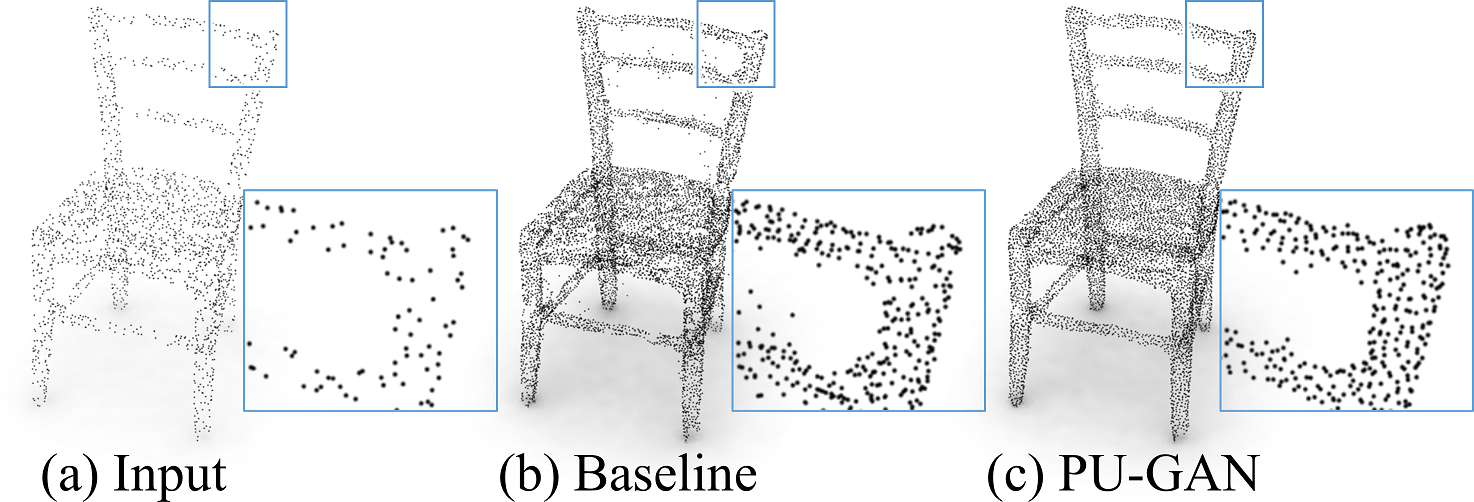
\includegraphics[width=1.0\linewidth]{baseline}
	\caption{Visual comparison of (c) PU-GAN against (b) the baseline GAN model, given (a) an input of 2,048 non-uniform points.}
	\label{fig:baseline}
	\vspace*{-2mm}
\end{figure}



%As Table ~\ref{tab:ablationStudy} shows, all components contributes positively to the full model. In particularly, the adversarial training can significantly boost the performance of upsampling procedure. Integrated attention module and uniform loss considerably promote the upsampling results and the farthest sampling improves performance slightly. After replacing the proposed up-down-up expansion unit with one up expansion, the uniformity of the generated points will be affected by a large negative impact.


\subsection{Other Experiments}

%\para{Upsampling with different noise levels.} \
%We investigate the robustness of PU-GAN by applying it to inputs of different noise levels.
%Figure~\ref{fig:noise} shows the comparison results with MPU~\cite{yifan2018patch}, where the inputs are corrupted by increasing amount of Gaussian noise, indicating that PU-GAN can still generate a satisfying upsampling result even under large noise corruption; see particularly the blown-up views.
%Please refer to our supplemental material for results under more continuous noise levels.
%can still generate a satisfying upsampling result even under large noise corruption.

\para{Upsampling point sets of varying noise levels.} \
Figure~\ref{fig:noise} shows the results of using PU-GAN to upsample point sets of increasing Gaussian noise levels, indicating the robustness of PU-GAN to noise and sparsity.
Please refer to the supplemental material for more results.

\para{Upsampling point sets of varying sizes.} \
Figure~\ref{fig:diff_point_num} shows the results of upsampling input point sets of different sizes; our method is stable even for input with only 512 points; more results are shown in the supplemental material.

\para{Applications.} \
Besides surface reconstruction and rendering (see Figure~\ref{fig:visualComparison}), point cloud upsampling is also helpful for object recognition.
To demonstrate this, we trained PointNet (vanilla version)~\cite{qi2016pointnet} on ModelNet40 dataset~\cite{wu20153d} for classification under two cases:
in case (i), we directly trained PointNet to take sparse training set (512 points) as inputs for classifying objects in the sparse testing set;
and in case (ii), we upsampled the point clouds in both sparse training and testing sets to 2,048 points using PU-GAN and then trained another PointNet with the upsampled training set for classifying the upsampled data in the testing set.
Results show that, the overall classification accuracy increased from 82.4\% (case (i)) to 83.8\% (case (ii)), indicating that PU-GAN helps improve the classification performance.


\begin{figure}[!t]
	\centering
	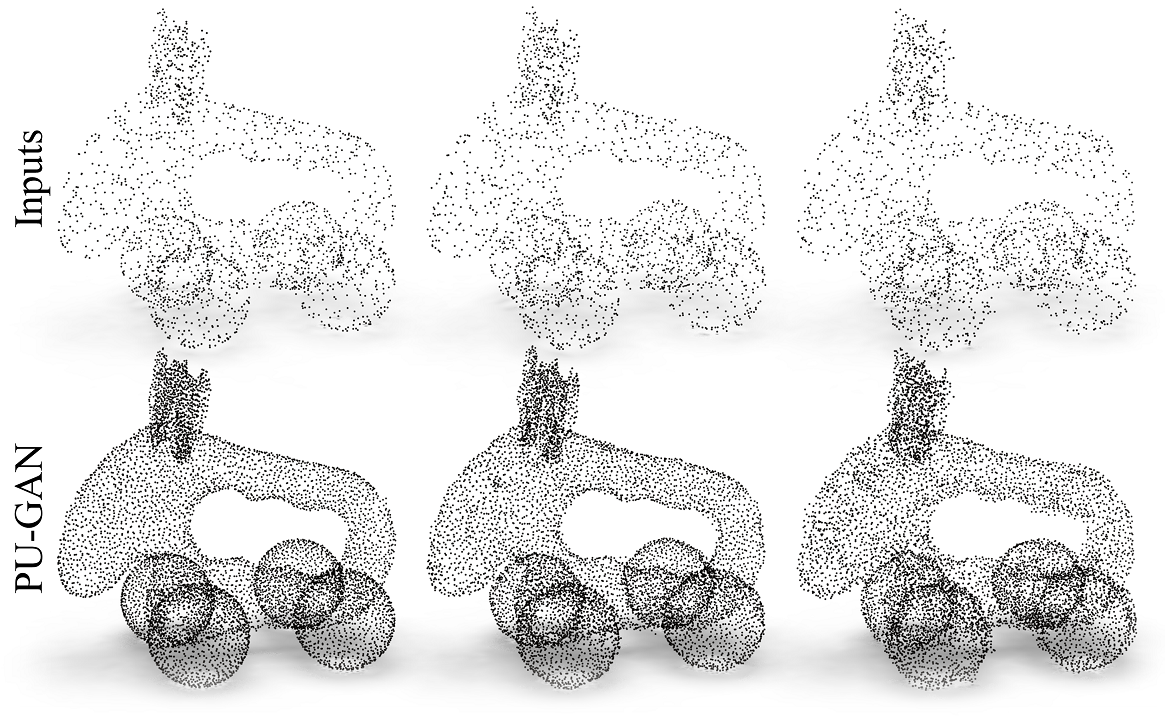
\includegraphics[width=1.0\linewidth]{noise}
	\vspace{-4mm}
	\caption{Upsampling results by applying PU-GAN to inputs with noise level of 0, 0.5\%, and 1\%.}
	\label{fig:noise}
	%\vspace*{-2mm}
\end{figure}

\begin{figure}[!t]
	\centering
	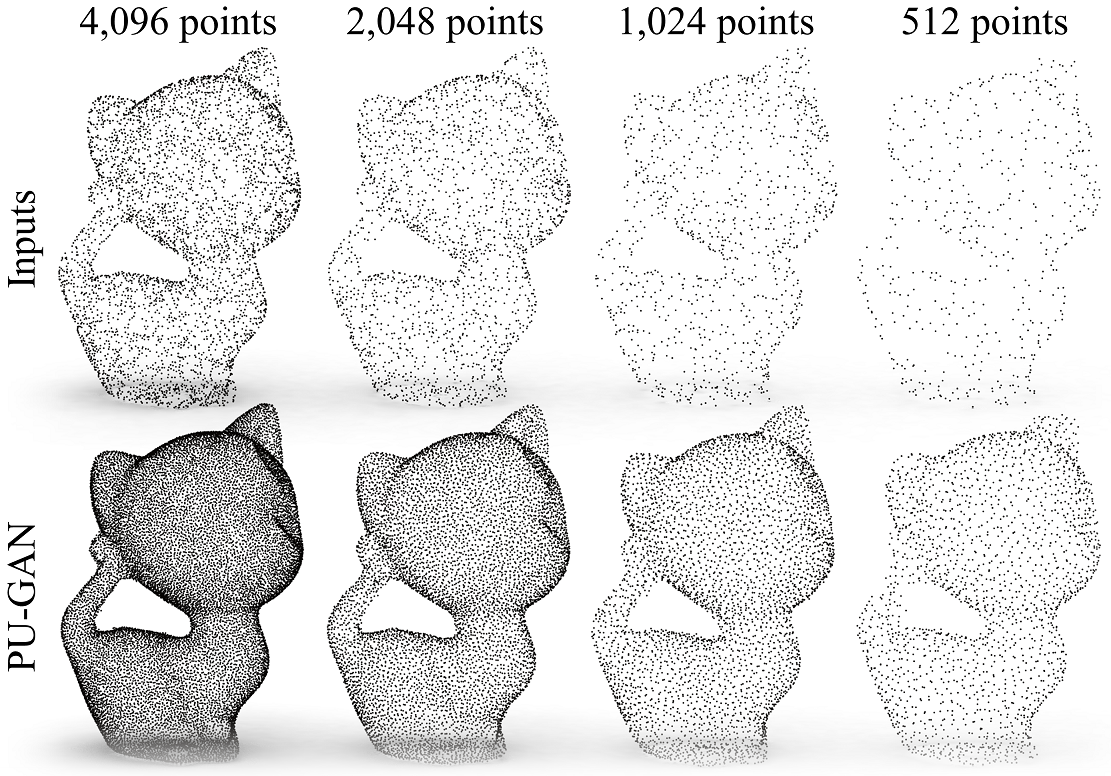
\includegraphics[width=1.0\linewidth]{diff_point_num}
	\vspace{-4mm}
	\caption{Upsampling point sets (top row) of varying sizes.} % 512,1024,2048,4096.}
	\label{fig:diff_point_num}
	\vspace*{-2mm}
\end{figure}


%\begin{table}[t]
%\centering
%	\caption{Classification accuracies by using PointNet on ModelNet40 dataset under case (i) with sparse point sets and case (ii) with our upsampled point sets.}
%	\label{tab:classification}
%\begin{tabular}{c|ccc}
%\toprule[1pt]
%ModelNet10                      & Case(i) & Case(ii) \\ \hline
%overall classification accuracy & 82.4\%    & 83.8\%     \\
%average class accuracy          & 76.7\%    & 77.8\%     \\
%\bottomrule[1pt]
%\end{tabular}
%\end{table}


\if 0
\subsection{Limitation}
\label{subsec:limitation}
As shown in Figure \ref{fig:limitation}, when there are some large gaps(\eg, head) among the given inputs, the proposed model just generate points around these holes, but can not fully complete the surface. And For which extremely sparse areas(\eg, foot), the produced results maybe noisy.

\begin{figure}
	\centering
	\includegraphics[width=1.0\linewidth]{limitation}
	\caption{Limitation for the proposed PU-GAN}
	\label{fig:limitation}
\end{figure}
\fi 
\section{Conclusion}
\label{sec:conclusion}
%In this paper, we presented a new network based on GAN for point cloud upsampling, namely PU-GAN, to generate dense and uniformly-distributed points from sparse and non-uniform inputs. In particular, we direct the attention of the proposed network to global uniformity by introducing an up-down-up expansion unit, a self-attention module and a uniform loss into the generator. These integrated modules can enhance the uniformity of generative distribution and promote the discriminator to learn more latent patterns. Such adversarial training enable us to generate highly uniform point distribution. Extensive experimental results demonstrate the superiority of our PU-GAN compared with the state-of-the-art approaches.

In this paper, we presented, PU-GAN, a novel GAN-based point cloud upsampling network,  that combines upsampling with data amendment capabilities.
Such adversarial network enables the generator to produce a uniformly-distributed point set, and  the discriminator to implicitly penalize outputs that deviate from the expected target.
To facilitate the GAN framework, we introduced an up-down-up unit for feature expansion with error feedback and self-correction, as well as a self-attention unit for better feature fusion.
Further, we designed a compound loss to guide the learning of the generator and discriminator. We demonstrated the effectiveness of our PU-GAN via extensive experiments, showing that it outperforms the state-of-the-art methods for various metrics, and presented the upsampling performance on real-scanned LiDAR inputs.

However, since PU-GAN is designed to complete tiny holes at patch level, it has limited ability in filling large gaps or holes in point clouds; see Figure~\ref{fig:realscan}. Analyzing and synthesizing at the patch level lacks a global view of the overall shape.
\rh{Please refer to the supplemental material for a typical failure case.}
In the future, we will explore a multi-scale training strategy to encourage the network to learn from both local small patched and global structures.
We are also considering exploring conditional GANs, to let the network learn the uniformity and semantic consistency at the same time.

%In this paper, we presented a novel GAN based point cloud upsampling network, namely PU-GAN, that combines upsampling with data amendment capability.
%Such adversarial network enables the generator to produce a uniformly-distributed point set, and also the discriminator to implicitly penalize outputs that deviate from the target.
%To facilitate a working GAN framework, we introduced an up-down-up expansion unit for feature expansion with error feedback and self-correction, as well as a self-attention unit for better feature fusion.
%Further, we designed a compound loss to guide the learning of the generator and discriminator.
%We demonstrated the effectiveness of our PU-GAN via extensive experiments, and presented the promising upsampling performance on real-scanned LiDAR inputs.

%However, it cannot be ignored that our method has limited ability to fill in large gaps, despite the fact that it can complete tiny holes at patch level; see Figure~\ref{fig:realscan}.
%We think that this may be related to the patch-based training strategy, since it lacks the global information.
%In the future, we would like to employ a dynamic patch size training strategy to enforce the network to learn from both local details and global structures.
%Further, we may also explore other advanced GAN framework,~\eg, conditional GAN~\cite{mirza2014conditional}, to enforce the network to learn the uniformity and semantic consistency as the same time.
%extend the proposed network with the Condition GAN  enforce prediction in the same semantic space as the inputs. And we also try to extend the current PU-GAN into point consolidation or completion under the additional constrain, such as single-view images or point-to-edge distances. 

\para{Acknowledgments.} \
We thank anonymous reviewers for the valuable comments.
The work is supported by the 973 Program (Proj. No. 2015CB351706), the National Natural Science Foundation of China with Proj. No. U1613219, the Research Grants Council of the Hong Kong Special Administrative Region (No. CUHK 14203416 \& 14201717), and the Israel Science Foundation grants 2366/16 and 2472/7.

{\small
\bibliographystyle{ieee}
\bibliography{egbib}
}

\end{document}
